% This is samplepaper.tex, a sample chapter demonstrating the
% LLNCS macro package for Springer Computer Science proceedings;
% Version 2.20 of 2017/10/04
%
\documentclass[runningheads]{llncs}
%
\usepackage{graphicx}
\usepackage[portuges]{babel}
\usepackage[T1]{fontenc}
\usepackage{verbatim}
\usepackage{float}
\usepackage{listings}
%Path relative to the .tex file containing the \includegraphics command
\graphicspath{ {./images/} }
% Used for displaying a sample figure. If possible, figure files should
% be included in EPS format.
%
% If you use the hyperref package, please uncomment the following line
% to display URLs in blue roman font according to Springer's eBook style:
% \renewcommand\UrlFont{\color{blue}\rmfamily}
\setcounter{secnumdepth}{6}
\renewcommand\theparagraph{\Alph{paragraph}}
 
\makeatletter
\renewcommand\paragraph{\@startsection{paragraph}{4}{\z@}%
                                      {-3.25ex\@plus -1ex \@minus -.2ex}%
                                      {0.0001pt \@plus .2ex}%
                                      {\normalfont\normalsize\bfseries}}
\renewcommand\subparagraph{\@startsection{subparagraph}{5}{\z@}%
                                      {-3.25ex\@plus -1ex \@minus -.2ex}%
                                      {0.0001pt \@plus .2ex}%
                                      {\normalfont\normalsize\bfseries}}
 

\makeatother


\begin{document}
%
\title{MSTG - Teste de aplicações Android e iOS}
%
%\titlerunning{Abbreviated paper title}
% If the paper title is too long for the running head, you can set
% an abbreviated paper title here
%
%\author{Adriana Lopes \and Diana Carrilho \and Henrique Faria \and Paulo Barbosa}
\author{}
%
% First names are abbreviated in the running head.
% If there are more than two authors, 'et al.' is used.
%
\institute{Departamento de Informática, Universidade do Minho}
%
\maketitle              % typeset the header of the contribution
%
% Abstract
\begin{abstract}

\keywords{MSTG  \and Android \and iOS.}
\end{abstract}
%
%
% Introdução
\begin{center}
\normalsize{\bfseries Introdução}\hfill 
\end{center}








\newpage
\hfill
% Aqui começam os capitulos abordados pelo trabalho

% regra de adição -> \input{ficheiro a adicionar pela ordem certa}
%\input{}
\section{OWASP Mobile Security Testing Guide}

	O MSTG é uma guia/manual que descreve como verificar os requisitos listados no MASVS (Mobile Application Security Verification Standard). Descrevendo várias tecnicas gerais e especificas para o sistema operativo de como fazer Tests aos requisitos. Este livro teve vários autores, co-autores, colaboradores grandes e pequenos visto que é um livro open source. Os autores principais são Bernhard Mueller, Jeroen Willemsen e Sven Schleier.
	Seguidamente, serão feitos alguns pontos importantes sobre a natureza das aplicações, hardware onde estas aplicações executam.
	Mobile Apps tem uma superficie de ataque menor, isto é, menos vetores de ataques possíveis do que um sistema completo. Assim prioritiza-se a proteção da informação contida nas Apps e as suas ligações com a rede.
	O cuidado a ter com a informação guardada deve ser grande visto que facilmente os "telemoveis" são robados fisicamente, e também, comunicam com vários sistemas. Isto implica que deve-se usar com precaução as APIs do Sistema Operativo e de IPC( Inter-process Communication) para evitar desvelar informação a outros processos a correr na mesma máquina ou para um sistema de Cloud storage, cache ou similar. Assim, recomenda-se usar APIs recomendada para guardar as Key criptograficas e HSM (Hardware Security Module) se tiverem disponiveis nas últimas versões mesmo que isto implique excluir utilizadores. Em termos de comunicação com o exterior recomenda-se usar protocolos seguros como são o SSL/TLS.
	Ao nivel aplicacional, deve-se ter em contas as vantagens e desvantagens dos diferentes tipos de autentificação sejam estes implementados pelo próprio serviço ou ainda utilizando frameworks de autentificação como OAuth2 (Google, Facebook, Twitter ....). Tendo especial cuidado as APIs especificas que contem os seus próprios problemas e cuidados a ter seja Android ou iOS.
	A comunicação usada pelas aplicações é, na sua maioria, isolada. Assim, estas são mais resistentes a buffer overflow vulnerabilities e XSS (Cross-site Scripting) attacks. Dito isto, ainda se requere que o código siga as melhores práticas para fortalecer a segurança e, por conseguinte, evitar tampering.

\section{Terminologia}

	Nesta seção apresentar-se-á vários conceitos fundamentais para entender o contexto de analise e teste de uma aplicação. O primeiro considera o conhecimento do teste sobre a aplicação a testar, divindo em três conceitos:

\begin{itemize}

\item Black-Box Testing - O tester/test apenas conhece a informação pública sobre a aplicação comportando-se o mais próximo possível de um atacante real.

\item White-Box Testing - Oposto do anterior, o tester conhece a aplicação por completo, isto é, source code, funcionalidades, documentação, diagramas, etc.

\item Gray-Box Testing - Meio-termo. É o mais comum na industria visto que compromete-se no número de testes, etc. Também se compremete no conhecimento disponibilizado ao tester, sendo um compromisso entre o tempo,da completude dos testes.

\end{itemize}

Recomenda-se para um aplicação que não foi testada ainda que se use o White-Box Testing para detetar os problemas de segurança ao nivel do código. Sejam estes ao nivel de segurança ou ao nivel lógico de funcionamento.

A analise destas vulnerabilidades pode ser feita de das seguintes formas:

\begin{itemize}

\item Static Application Security Testing (SAST) - Esta tecnica examina os componentes da aplicação analisando o source code manualmente ou atraves de uma ferramenta que o faça automaticamente. A analise manual pode ser feita de várias maneiras usando metodos como grep para procurar certos comandos especificos que se conheça que possa conter vulnerbilidades. Por exemplo, funções que acedam a uma base de dados. De forma a ajudar o processo pode se usar algumas ferramentas que apontam para possiveis problemas ( IDE + Tools). É útil para quando se quer encontrar problemas lógicos no programa, falhas no design, etc. No entanto este tipo de review é lenta, consome bastante tempo e requer alguem que seja proeficiente tanto na linguagem como nas ferramentas usadas.A analise automatica permite complementar a analise manual. Aponta para problemas e avisos seguindo algumas regras configuradas na ferramenta usada. Os problemas tem que ser revistos por um professional já que é possível haver falsos positivos.

\item Dynamic Application Security Testing (DAST) - Esta tecnica analisa a aplicação enquanto esta está a executar. Principalmente, obtendo informação sobre falhas de segurança não no código mas na interação das varias componentes do mesmo. Por exemplo,encontrar vulnerabilidades no processo de auntentificação e autorização ,como nos padrões dos pedidos e respostas entre ambos os intervenientes,erros de configuração no servidor, etc.


\end{itemize}

O Pentesting consiste em utilizar um leque de ferramentas para testar eludir a segurança implementada na aplicação. É recomendado a utilização do MASVS como base para o teste. A seguir apresenta-se uma lista de passos que devem ser seguidos para os testes procederem com normalidade e efetivamente.

\subsection{Preparation}

	Processo necessário antes de começar os testes. Definir o que se quer testar, que controis de segurança, objetivos dos testes, sensitive data. Acordar com o Cliente o que se pretende fazer requererndo uma autorização escrita para definir os limtes. Os testes a ser realizados, a cobertura dos mesmos e os requisitos que se quer cumprir da lista do MASVS tem que ser discutido com o cliente. Apesar da lista do MASVS Level 1 ser aplicável para as Mobile Apps, o melhor é comunicar com os skateholders. Enquanto ao L2 é necessário rever quais as leis e os regulamentos que podem ser aplicados ao tipo de aplicação que se pretende desenvolver visto que estes requisitos são para aplicações mais criticas.
	Todas as decisões tomadas sobre os requisitos de segurança a serem desenvolvidos/testados tem que ser acordados com o Cliente como justificados num relatorio. Tanto para evitar problemas legais com o mesmo como também para testar todos os requisitos necessários.
	É possivel que existam outras restrições para os testes para a analise dinamica nas instalações do cliente. Por exemplo, não permitirem usar ferramentas de analise da rede por parte do cliente. Uma forma de testar seria usar o Black Box testing para a analise dinamica e requisitar a aplicação em release e em modo debug com algumas funcionalidades desativadas de forma a poder testar os vários requisitos de segurança.
	Outro ponto importante é identificar qual é que é considerado informação sensivel que a aplicação manipula. Para ser possivel testar se existe algum tipo de leak sobre esta informação.Caso não haja um acordo sobre este ponto podem ser considerados os seguintes pontos:

\begin{itemize}

\item Informação de autentificação do utilizador (credenciais, PINs, etc.).

\item Informação que possa ser utilizada para identificar a pessoa, podendo ser utilzada para realizar um roubo de identidade.

\item Informação que apesar de produzida pela aplicação, tem que ser protegida ao abrigo das leis.

\item Informação gerada pela aplicação que é importante para a segurança da aplicação e/ou do próprio sistema.

\end{itemize}

\subsection{Intelligence Gathering}

O processo de recolha de informação deve recolher informação ambiental, isto é, do contexto onde é executada como informação arquitetural. Como informação do primeiro tipo pode ser considerado o seguinte:

\begin{itemize}

\item Os objetivos da aplicação
\item O perfil de risco da aplicação
\item Skateholders e investidores

\end{itemize}

E, como informação arquitetural:

\begin{itemize}

\item Acesso de informação pela aplicação, comunicação com outros processos, gestão das sessões de utilzadores, deteção e reação de jailbroken e rooted phones.

\item Sistema Operativo e versão do sistema operativo em qual a aplicação vai correr. Se é esperado correr em dispositivos que tenhas mobile device Management(MDM) controls e outras vulnerabilidades do sistema operativo.

\item NETWORK: Como usa a rede? Usa protocolos seguros? Usa chaves de tamanho suficiente e algoritmos fortes?

\item Remotes Services: Quais os serviçoes remotos que aplicação usa e se um ataque aos mesmos pode afetar a aplicação.

\end{itemize}


\subsection{Mapeameanto da Aplicação}

Após o security tester ter suficiente informaçao sobre a aplicação como tambem do seu contexto pretende mapear a mesma, ou seja, identificar a estrutura da aplicação, os dados, os pontos de entrada e as funcionalidades. Para tal pode usufruir da documentação existente da aplicação, como , por exemplo, diagramas da arquitetura, especificação funcional, código. De forma a ajudar o security tester é aconselhavel as empresas realizarem Threat Modeling \cite{ref_intro7}. 

Para realmente, realizar o mapeameamento em conjunto com a documentação supra-citada deve-se utilizar tecnicas de SAST, caso seja possivel. E DAST para detetar as os aspetos acima citados como vulnerabilidades seja manualmente ou utilizando ferramentas.

\subsection{Exploitation}

O tester irá testar explorar as vulnerabilidades encontradas nas fases anteriores e analisa-las. Apesar de raramente se chegar a esta fase, permite classificar segundo varias dimensões as vulnerabilidades encontradas. As dimensões normalmente consideradas são as seguintes:

\begin{itemize}

\item Damage potential - o dano resultante de explorar esta vulnerabilidade.
\item Reproducibility - facilidade de reprodução do ataque
\item Exploitability - facilidade para executar o ataque
\item Affected users - O número de utilizadores afetados pelo ataque
\item Discoverability - Facilidade de descoberta da vulnerabilidade

\end{itemize}

\subsection{Reporting}

Todas as vulnerabilidades deve ser devidamente documentadas para que o Cliente perceba qual o impacto da vulnerabilidade encontrada. Existem muitos tipos de templates para fazer report do testing feito. Por exemplo, qual a vulnerabilidade, com que teste foi encontrado, como é que o teste foi executado, a possibilidade da vulnerabilidade ser explorada, o que é comprometido caso seja explorado são só alguns exemplos de dados que podem estar na documentação.

\section{ SDLC - Software Devolpment Life Cycle }

O ciclo completo de SDLC consiste em vários passos que podem ser incorporados num paradigma Waterfall ou no paradigma Agile. Isto é, podem ser adaptados a paradigmas que fazem passo a passo ou incrementais.

\begin{itemize}

\item Risk Assessment - Realizar perfis dos riscos para as diferentes componentes das aplicações. Para tal precisa-se ter em conta o tipo de informação que é armazenada e processado pela aplicação como os regulamentos adjacentes aos mesmos. Ainda deve-se ter em conta se a aplicação pode ser acedida Online ou não. Aqui poderia ser útil as politicas de classificação dos dados tratados.

\item Security Requirements - São determinados em conjuntos dos requisitos funcionais. Pode ser usado o OWASP MASVS para determinar esses requisitos para uma aplicação de telemovel.

\item Secure Design - Threat Modeling - Invés de analisar os assets que tem mais riscos como na fase de risk assessement aqui, enumera-se, identifica-se, classificando conforme a prioridade, e se possível propõem-se possiveis soluções para as Threats encontradas. Podendo ser estabelecidas regras para realizar código seguro, como também as ferramentas e método para realizar os testes de Segurança. Deve-se manter registo e documentação de todos as alterações e novos requisitos determinados em prol da segurança da aplicação. É sugerido que junto com os requisitos junte-se code snippets em vez de guiar o developer por palavras.

\item Secure Implementations - Security Code Reviews, SAST e Secure Unit Testing fazem parte desta fase.

\item Secure Testing -  Seguidamente, aquando da saida do código candidato para release deve-se realizar testes de PenTesting Manual e automaticamente como também DAST.

\item Aceptance/Secure Operations - Passa-se para os skateholders e caso estes aceitem o software, pode transitar para a fase de produção. Passando para equipa de Operações.

\item Decommissioning -  Finalmente, quando acabar a vida útil do software tem que se fazer o Decommissioning, isto é, removido tudo o que se possa em relação a esta aplicação.

\end{itemize}

Note-se que estas fases podem ser adaptadas e/ou omitidas.

\begin{figure}[h!]
\centering
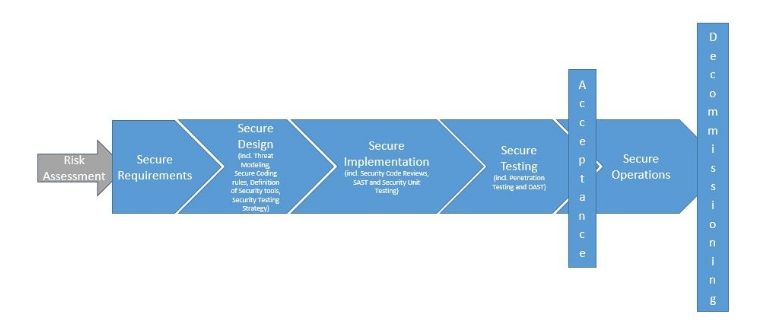
\includegraphics[width=\textwidth]{SDLC.png}
\label{fig:sdlc}
\caption{SDLC}
\end{figure}


\subsection{Definindo uma estrategia de Teste}

	Uma estrategia de teste deve definir quais os tipos de testes a serem realizados como a frequência dos mesmos. Esta estrategia costuma ser definiada apos serem clarificados os riscos e antes da implementação. Outro Input importante é o Threat Modeling executado.
	A estrategia deve ser partilhada pelas diversas equipas envolvidas no projeto visto que a equipa que o define pode nao ser a que a implementa ou pode causar conflitos com algumas delas.
	Para alem de definir quais os testes a serem realizados também define os objetivos com os testes, a descrição dos riscos definidos na fase anterior como qual a importancia dos testes(obrigatorios ou opcionais), quando e como serão executados.
	Para além disso deve-se manter metricas para analisar se a estrategia definida está a ser efetiva. Algumas metricas possiveis são:

\begin{itemize}

	\item Code coverage para os testes unitarios de security controls
	\item Número de bugs de segurança encontrados em cada build apos analise via ferramentas de analise estatica de código.
	
\end{itemize}


\subsection{Security Testing in Waterfall - Agile}

	O modelo Waterfall é sequencial o que causa que os testes, e correção das vulnerabilidades encontradas só irá acontecer depois da aplicação ser desenvolvida e estes erros serão corrigidos com poucas mudanças a arquitetura da aplicação.

	O modelo Agile requer evoluções incrementais do software, ou seja, entregas e desenvolvimento de software. A seguir ir-se-á falar de um cargo importante neste paradigma de software.
	O DevOps é um cargo que implica a colaboração com a equipa de desenvolvimento (DEV) e com a equipa de Operations(OPS). De forma a agilizar o processo de deployment de software, automatizando o processo de build, o processo de testes, de release de softwares e mudanças na infraestrutura(CI/CD). Atualmente, este cargo está a evoluir de tal forma que precisa de colaborar com várias equipas envolvidas no projeto como a equipa de qualidade, de segurança etc... 
	Tendo em vista, o foco principal desta guia focar-se-á no DevSecOps, isto é, adicionar segurança ao processo de DevOps. Os DevSecOps foca-se em minimizar o numero de defeitos da aplicação antes de chegar a produção. Mas também, monitorizar o processo da equipa de Operations para identificar problemas que podem realimentar o processo de desenvolvimento. Dando assim enfase no processo de CI.

	Com o objetivo de conseguir acompanhar a rapidez do processo, necessita-se automatizar o processo principalmente os sub processos essenciais. E abandonar as tarefas que não são produtivas. Focando-se em tres aspetos principais:

\begin{itemize}

\item Infraestructure as Code - A infraestrutra é mantida atraves de scripts, ficheiros de configuração mantidos sobre version control para facilitar partilha e resoluçao de problemas. Por exemplo, ficheiros de configuração para Dockers, maquinas virtuais, etc. Assim, facilita a construção de ambientes de desenvolvimento para as diferentes equipas envolvidas no processo de criação de software.
Alguns recursos Cloud-based providenciam APIs para aceder a items como maquinas virtuais, espeaço de armazenamento e configurações.Ferramentas usadas Puppet, Terraform, Packer, Chef and Ansible.

\item Deployment - A sofistificação do pipeline depende da maturidade da equipa de desenvolvimento. A commit phase normalmelmente involve compiler checks junto com os unit tests associados. Atraves deste sistemas providencia um sistema de feedback para os developers. 
Continuos Integration - Usa o código disponivel para construir o candidato de release. A seguir realiza-se os testes necessários e se forem confirmados pode passar a fase seguinte.
Continuous Delivery -  Após o candidato de release ser avaliado e validado (manual ou automaticamente) o deployment pode continuar.
Continuous Deployment - As releases são passadas para produção sendo disponibilizadas para o utilizador.

\item Security - Os testes de analise estaticos de aplicação podem ser integrado no processo de CI utilizando ferramentas para automatizar o processo. Estabelecendo também Secure Coding Rules. Aquando da release pode ser realizado testes de DAST e, também depois de cada build. Ainda pode-se juntar mais testes manuais no meio das fases. Na fase de Operations deve-se realizar regularmente scans, Pentesting e monitorização ativa de forma de ativar o loop de Feedback.

\end{itemize}

\section{Mobile App Authentication Architectures}


	Os problemas mais prevalentes em termos de segurança são a autentificação e a autorização. Tal pode ser confirmado visto que aparecem no OWASP Top 10 \cite{ref_intro8} em segundo lugar várias vezes.
	Apesar de parte da autentificação e gestão do estado serem mantidos no servidor de backend é importante estudar as implementações mais comuns que podem ser incorporadas em aplicações moveis.
	O tipo de autentificação mais indicada para uma aplicação depende do contexto da mesma, onde vai ser executada, quais os regulamentos que tem de obedecer, etc... Por exemplo, Apps para redes sociais, forums ou similares basta um par username / password com as devidas recomendações para utilização de passwords fortes. Enquanto que uma aplicação com acesso a informação sensivel como é o caso de um banco deve usar 2FA (2-Factor-Authentification) como username/password mais SMS Token. Outra guia possível como já foi referido é usar o MASVS Level 1 para aplcações não criticas e o Level 2 para o outro tipo.
Adicionalmente, pode usar-se a GeoLocation, IP adress e o dispositivo usado para encontrar desvios de comportamento que podem assinalar que a conta do utilizador pode ter sido roubada ou tentativas de fraude.

\subsection{MSTG-ARCH-2 e MSTG-AUTH-1}

Uma das propriedades importantes para testar na autentificação e autorização é se está implementada nos locais corretos. Para tal é preciso ser feito:

\begin{itemize}

\item Identificação de todos os processos de autentificação que aplicação usa.
\item Localização onde estão os endpoints que fornecem uma funcionalidade critica
\item Verificação que existe concordância entre todos os processos de autentificação e os endpoints antes referidos

\end{itemize}

Os servidores devem verificar que o utilizador estã autentificado cada vez que estes requerem um recurso do servidor. Seja atraves das sessões mantidas no servidor ou dos Tokens junto com signatures. Desta forma consegue-se evitar o tampering.

\subsection{MSTG-AUTH-5 e MSTG-AUTH-6}

As passwords usadas pelos utilizadores devem ser fortes para tal deve se implementar uma politica de password. Esta deve obrigar aos utilzadores a escolherem password que cumpre certo número de requisitos de forma a impedir o cracking da password através de métodos manuais ou automáticos.

A OWASP criou uma lista de requisitos para as complexidades das passwords de forma a garantir a segurança das mesmas \cite{ref_intro9}.

Para além disso recomenda-se mostrar os utilzadores a "força" das suas password quando as estão a escolher utilzando bibliotecas como o zxcvbn.

\subsubsection{Login Throttling}

Os atacantes pode tentar descobrir as credenciais de acesso atraves de Brute Force para evitar o mesmo deve ser implementado algumas das seguintes práticas:

\begin{itemize}

\item Bloquear contas temporariamente/permanentemente depois de muitas tentativas falhadas de Login (por exemplo os bancos)

\item Os controls para impedir brute-force deve ser implementados ao nivel do servidor visto que quando implementados ao nivel do cliente podem ser facilmente bypassed.

\item Um conjunto maior de tecnicas para evitar brute force pode ser encontrado no seguinte link da OWASP \cite{ref_intro10}.

\item É so de notar que os sistemas de bloqueio de contas podem causar problemas como DoS para várias contas.

\end{itemize}

Uma forma para testar dinamicamente este sistema de passwords é usar programas como o OWASP ZAP para definir ataques de Brute Force com Dicionario. Para testar contas que se conheça a password utiliza-se uma lista de passwords em que no final está a correta. Caso após algumas tentativas não exista nenhum tipo de bloqueio, temporizador ou captcha pode se concluir que o sistema está suscetivel a ataques por brute-force.


\subsection{MSTG-AUTH-2 e MSTG-AUTH-7}

As Autentificação Session-based pode sofrer ataques de tampering vários por isso também devem ser testados, antes de começar com os cuidados, ir-se-á explicar o fluxo:

1 - App envia um request com as credenciais do utilizador para o servidor

2 - Verifica as credenciais, caso estas sejam válidas uma nova sessão é criada com uma ID gerado aleatoriamente para a sessão.

3 - O servidor envia a resposta que inclui esse ID.

4 - Todas as requests feitas pelo cliente após a auntentificação é adjunto esse Session ID. E o servidor valida e recupera o record associado com essa sessão.

5 - No momento em que o utilzador fizer log out  o record mantido pelo servidor é destruido e o utilizador apaga o Session ID.

Estas sessões devem ser devidamente gerenciadas sendo recomendado o uso de frameworks especializadas no mesmo. Sempre com atenção para os seguintes pontos:

\begin{itemize}

\item Session IDs são gerados aleatoriamente
\item Session IDs são imprevisiveis
\item Session IDs são trocados usando secure connections (HTTPS)
\item Session IDs não são guardados no armazenamento permanente ("Disco")

\end{itemize}

Para complementar o teste a aplicação movel, pode realizar teste ao servidor de back-end seguindo o OWASP Web Testing Guide \cite{ref_intro11} \cite{ref_intro12}

O tempo de vida das sessões devem ser limitado conforme a natureza da aplicação onde vai ser usada. Caso haja acesso ao código pode-se verificar diretamente, caso contrário atraves de um proxy faz-se login numa conta, tenta-se aceder a um recurso tipicamente protegido cada 5 minutos. Quando o servidor devolver um timeout signfica que o timeout está nesse intervalo de 5 minutos. Caso o tempo seja demasiado longo ou inexistente o teste falha. Os tempos de timeout devem pertencer ao intervalo [10, 120] minutos dependendo da aplicação.

\subsection{MSTG-AUTH-4}

O logout incorreto do utilzador é uma falhas mais comuns encontradas. Apesar de ser uma falhas simples pode permitir hijack da conta do utilzador. Isto é possível visto que as sessões não foram devidamente destruidas e os tokens invalidados.

Para testar, caso o código esteja disponivel, deve-se rever a implementação e compara-la com soluções de referência. Caso queira-se fazer uma analise dinamica pode testar fazendo o seguinte:

1 - Log in

2 - Aceder a recurso protegido

3 - Log out

4 - Tentar aceder ao mesmo recurso protegido

A resposta após Log out deve ser um redirecionamento ou um código de erro. Caso contrário significa que o sistema não destroi as sessões / invalida os tokens como pretendido.

\subsection{MSTG-AUTH-9 e MSTG-AUTH-10}

Two-Factor Authentification (2FA) é usada para aplicações que acedem a dados/funções que devem ser mais protegidos. Normalmente, um user/password para o primeiro passo da auntentificação e alguns dos seguintes como segundo:
\begin{itemize}

\item One-time Password via SMS (SMS-OTP)
\item One-time code por chamada telefonica
\item Hardware/Software Token
\item Push notifications em combinação com PKIs

\end{itemize}

Primeiro,e apesar de ser uma prática normal, o uso de SMS-OTP apresentam várias ameaças. Entre elas estão:

\begin{itemize}	

\item A utilização de femtocells para interceptar os SMS

\item Trojans instalados no próprio dispositivo que possa transmitir a mensagem para o dispositivo do atacante, por exemplo.

\item SIM SWAP Attack, isto é, conseguir pedir uma segunda via do cartão SIM pelo atacante.

\end{itemize}

Os problemas anteriores podem ser mitigados ou dificultados para o atacante para tal sugere-se usar alguns dos seguintes mecanismos:

\begin{itemize}

\item Usar o canal dedicado. Usar uma aplicação dedicada para receber este tipo de mensagens que não possam ser acedidas por outras aplicações.

\item Usar autentificadores com maior entropia de forma a fazer os OTPs mais dificeis de advinhar ou descobrir.

\item Utilizar Push Notifications em combinação com PKIs assinando as transações executadas. Exemplo de Funcionamento: A aplicação gera um par chave privada/publica e regista a publica no servidor de back-end. A chave privada é guardada na KeyStore/KeyChain. Finalmente para processar a transação, o servidor envia a informação da transação para o utilizador, este confirma-a, desbloqueia com uma password ou fingerprint o KeyStore/KeyChain de forma a obter a chave privada. De seguida, assina a transação com a chave privada, permitindo o servidor verificar com a chave pública.

\end{itemize}

	Um dos testes possíveis a segurança deste mecanismo seria testar os 2FA e interceptar as requests. Realizar replays attacks a partir das requests intercetadas. Testando se é possivel aceder a recursos defendidos por esta autentificação. Caso o sistema responda quer dizer que o sistema não é seguro.
	O OTP requere que se bloquei após varias tentativas falhadas. Uma forma de testar é antes de enviar o código correto enviar 10-15 tentativas erradas. Caso o sistema não bloqueie antes da correta é considerado inseguro.


\subsection{ MSTG-AUTH-3 }

A autentificação por tokens resulta de enviar tokens assinados/verificados pelo servidor com cada HTTP request. Estes tokens são divididos em três partes: o header, o payload e a assinatura.

O header é composto pelo nome do algoritmo usado e o tipo do token. O payload contem informação sobre o utilizador e metadata. O último valor é a assinatura que é calculada da forma Alg(header,payload,secret\_value). O segredo é partilhado entre o servidor de auntentificação e o servidor de backend ficando escondido do utilizador.

Numa perspetiva estatica de analise convêm verificar as seguintes propriedades como outros que não estão aqui listadas:

\begin{itemize}

\item Verificar que o HMAC é verificado em todos os requests que chegam.
\item Verificar que a chave privada como a chave secreta HMAC estão disponiveis só para o "emissor" da assinatura e o "verificador".
\item Verificar que os ataques por repetição são tratados pela utilização de JWT ID.
\item Verificar que os tokens são guardados seguramento no dispositivo como, por exemplo, KeyChain/KeyStore.

\end{itemize}

É importante que os Tokens tenham uma expiration date ou ainda implementar-se um esquema de acess tokens e refresh tokens.

Numa analise dinamica pode-se tentar fazer:
\begin{itemize}

\item Brute-Force da chave secreta offline utilizando ferramentas como John The Ripper.

\item Decodificar a base64 do JWT e verificar que tipo de informação é transmitida e se esta encriptada. É suposto que se existir informação sensivel esteja encriptada. 

\item Verificar se mudanças no header não resultam em Tokens validos com assinaturas forjadas.

\end{itemize}

\section{Cryptography for Mobile Apps}

\subsection{MSTG-CRYPTO-4}

Os algoritmos usados nas várias aplicações devem ser revistos com regularidade. Isto para que os algoritmos que estão a ser utilzados sejam alterados, o tamanho das chaves usadas atualizadas segundo as recomendações, as chaves são usadas cada uma para o seu propósito, isto é, a chave usada para HMAC deve ser diferente da chave usada para encriptação.

\subsection{MSTG-CRYPTO-1, MSTG-CRYPTO-2 e MSTG-CRYPTO-3}

A seguir apresenta-se vários conselhos que servem tanto para aplicações moveis como quase para qualquer tipo de aplicação que utilize mecanismos de criptografia.
\begin{itemize}

\item Assegurar-se que as chaves usadas nas aplicações não são guardados nos mesmos sitios que a informação que é encriptada/assinada/etc.

\item Recomenda-se não usar chaves estaticas compiladas diretamente no código visto que com ajuda de um disssambler consegues descobrir facilmente. A ofuscação do código também pode ser desfeita usando dynamic instrumentation.

\item A password do certificado deve ser guardada no Keychain caso sejam utilzados (Two-way SSL).

\item Uma forma de usar a password é usa-la como chave. Recomenda-se passar por uma KDF antes com pelo menos 10,000 iterações para gerar a chave a ser usada.

\item Deve-se evitar sempre o uso de funções criptograficas "caseiras" e optar por API Standard das plataformas escolhidas. As implementações não standard deve ser cuidadosamente analisadas, tendo em conta que os calculos intermedio de chaves e o estado interno da cifra tem que desaparecer da memória o mais rápido possivel.

\item Caso escolha-se o AES como encriptação deve-se escolher o modo de operação seguro, ou seja, evitar ECB, por exemplo. Seguir as recomendações sobre os IV/Nonces usados e ter em conta os ataques possíveis aos mesmos. E acompanhar com mecanismos de integridade, etc.

\item Escolher um bom mecanismo de Padding. Evitando o uso de PKCS\#5/7 e usar outros como o OAEP.  

\item Aquando do transporte de chaves entre dispositvos deve-se usar os mecanismos corretos. Por exemplo, criptografia assimetrica ou Key encapsulation mechanisms.

\end{itemize}

\section{Testing Code Quality}




O código tem que ser testado a sua qualidade visto que a mistura de frameworks e linguanges num projeto pode levar a algumas falhas como SQL Injection, buffer overflows e XSS.

\subsection{MSTG-ARCH-2 e MSTG-PLATFORM-2}

Uma falha de injeção de código refere-se quando algo que o utilizador escreve, seja isto diretamente do utilizador ou um processo é passado a um comando ou a uma query de backend resultando em comportamento não esperado.

Um caso tipico seria os casos de SQL Injection ou os XML Injection. Uma forma de testar passa pelo seguinte tendo em conta os canais mais perigos como a UI, IPC calls, QR Codes:

\begin{itemize}

\item Identificar entradas de untrusted Input e ver se é possivel executar funções que podem conter informação importante no alcance desse Input.

\item Identificar API e biblitecas que tenham comportamento perigoso caso o Input não seja devidamente visto ou "arranjado".

\item Deve-se usar Prepared Statments para separar a informação definida pelo o utilizador e o código.


\end{itemize}

\subsection{MSTG-CODE-8}

Os erros associados a corrupção de memória ate são comuns e pode ocorrer de várias formas. Os atacantes podem aproveitar-se disso para controlar o fluxo do programa e saltar certas condições de segurança ate injetar código pretendido. A seguir apresenta-se alguns problemas que causam este tipo de Bugs:

\begin{itemize}

\item Buffer Overflows - Descreve um erro que consistem em escrever depois de acabar o range de memória de certo objeto. Podendo apagar certas variaveis e apontadores para funções manipulando o fluxo como pretendido. Hoje em dia são mais raros porque já existe mais consciência sobre este tipo de problemas como também são faceis de detetar.

\item Use-after-free - Refere-se a utilização de pointers que apontam para memória já libertada. Podendo mais tarde este apontador referenciar outros objetos válidos.

\item Integer Overflows - Dependendo o que o inteiro represente pode ser útil para atacar o sistema provocar um Overflow ou Underflow.

\item Format String - Deixar o utilizador aceder as Formats Strings sem nenhum tipo de controlo pode causar em comportamento malicioso por parte do utilizador inserindo tokens para aceder a memória.

\end{itemize}

O teste para encontrar este tipo de vulnerabilidades pode ser intricado, mesmo usando ferramentas automáticas a não ser casos simples (RATS). Por isso, a forma mais eficaz de encontrar este tipo de vulnerabilidades é usar "Fuzzers" scripts que constroem estruturas semi bem formadas (Desde o Inicio ou mutando por uma estrutura antes válida). Envia-nas para a aplicação, ficando a escuta caso haja algum erro na aplicação. Cobrindo uma grande percentagem dos vários execution paths.

\section{Tampering and Reverse Engineering}

Reverse Engineering refere-se ao processo de analisar a aplicação compilada para extrair informação sobre o código fonte.Tampering refere-se ao processo de alterar a aplicação ou o ambiente de forma a afetar o comportamento da mesma. Por exemplo, alterar para poder correr certos tipos de testes.Ao misturar os dois pode-se moldar uma aplicação para realizar/permitir operações em prol do nosso interesse.Algumas vantagens do Reverse Engineering:
\begin{itemize}

\item Black-Box Testing - Apps modernas incluem mecanismo que previnem de interceptar or manipular trafégo com proxys ou Root Detection. Deve ser possivel desactivar essas defesas para realizar os testes.

\item De forma a facilitar a analise statica da aplicação. Ate pode-se encontrar credenciais hardcoded.

\item Para verificar a resistencia da própria aplicação ao reverse engineering. Para o tal o tester pode executar um resilience assessement como parte do teste geral de segurança.

\end{itemize}

\subsection{ Basic Tampering Techniques }

Binary Patching: alterar binarios já compilados, ficheiros por completo. Por exemplo, decompilar o código, editar e fazer re-assemble. Hoje em dia o processo é mais complicado porque o código vem assinado.Code Injection: modificar processos em execução atraves de ferramentas que permitem descobrir as library que estão loaded, funcões hooked, injetar código,etc . 

Existem várias ferramentas para realizar esta tarefa. Uma das mais versáteis e completas é a Frida.

A ferramenta, rapidamente, injeta código escrevendo diretamente na memória do processo. Atraves do ptrace faz hijack to processo, localizando o chunk de memoria. Seguidamente, carrega a library do agente da Frida e estabelece comunicação com a ferramenta. A thread volta ao fluxo normal apos de retornar ao estado original.

Para alem do funcionamento normal ainda existem mais modos disponiveis para execução desta ferramentas, como widgets e tools adicionais para acrescentar funcionalidades. Ou, ainda, outras ferramentas desenvolvidas a partir desta.

Disassemblers e Decompilers permitem reconstruir o código para um formato mais ao menos legivel para o tester. Assim, ganhando conhecimento de como o programa funciona e o fluxo que este tem.
Podendo juntar-se ao processo Debugging e Tracing para analisar o programa em execução, o primeiro para analisar o estado interno, definir breakpoints enquanto que o segundo permite recuperar informação sobre quais a execução da aplicação como as call a API.

\section{Testing User Interaction}

\subsection{MSTG-STORAGE-12}

Os utilizadores devem ser informados dos seus direitos, mais concretamente, do GDPR na Europa como os direitos associados ao mesmo. Como por exemplo, o direito a ser esquecido, o direito a correção da sua própria informação e o direito de aceder aos dados guardados pela aplicação sobre o utilzador.

Os utilizadores tambem deve ser informados dos perigos e melhores práticas de segurança sempre que pertinente.




%\definecolor{shadecolor}{rgb}{1,0.8,0.3}¹

%\title{Android}
%\author{Ricardo Vaz - PG41097 }
%\date{\today}

%\maketitle

%\tableofcontents

\newpage
\section{Arquitetura de Segurança do Android}
\begin{figure}[h!]
\centering
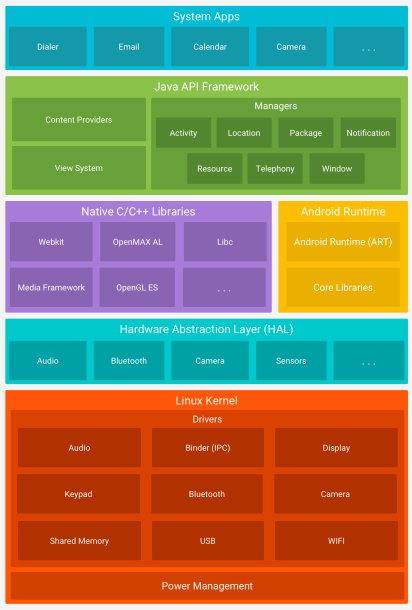
\includegraphics[scale=0.6]{arquiteturaAndroid.png}
\label{fig:arq}
\caption{Arquitetura}
\end{figure}

Android é uma plataforma Open Source baseada em Linux e desenvolvida pelo Google, que serve como um sistema operacional móvel.
Como é possível observar na figura \ref{arq}, esta é composta por várias camadas diferentes. Cada camada define interfaces e serviços específicos.


Uma das particularidas das aplicações Android, é o facto destas não terem acesso direto aos recursos de hardware e cada aplicação ser executada na sua própria sandbox, o que permite assim um controlo preciso sobre recursos e aplicativos, por exemplo, quando uma aplicação falha, esta não afetará as restantes aplicações em execução no dispositivo. Outra das particularidades do Android, é que o tempo de execução deste controla o número máximo de recursos do sistema alocados nas aplicações, impedindo, deste modo, que qualquer aplicação monopolize muitos recursos.



\section{Criptografia de dispositivos Android}
Este sistema operativo, suporta criptografia de dispositivo desde da versão 2.3.4 (API nível 10), e que desde então tem passado por grandes mudanças. Por imposição do Google, todos os dispositivos com Android 6.0 (nível 23 da API) ou superior passaram a ter que suportar criptografia de armazenamento, o que em alguns casos veio afetar significativamente o seu desempenho. Criptografia esta que se encontra dividida em três grupos: 
\\
\par \textbf{Full-Disk Encryption} 
Versões 5.0 (nível de API 21) e superiores oferecem suporte à criptografia de disco completo. Esta criptografia usa uma única chave protegida pela senha do dispositivo dos utilizadores para encriptar e desencriptar a partição de dados do utilizador. Este tipo de criptografia, nos tempos atuais, é considerada obsoleta, sendo que, a criptografia baseada em arquivo deve ser, preferencialmente, usada sempre que possível, visto que, a criptografia de disco completo apresenta desvantagens, como não poder receber chamadas ou não ter alarmes operacionais após uma reinicialização se o utilizador não digitar a senha para desbloquear.
\\
\par \textbf{File-Based Encryption}
A versão 7.0 (API nível 24) já suporta criptografia baseada em arquivo. Esta permite que arquivos diferentes sejam encriptados com chaves diferentes, para que possam ser desencriptados independentemente. Fazendo com que os dispositivos que suportam este tipo de criptografia também ofereçam suporte à Inicialização Direta. Esta permite que o dispositivo tenha acesso a recursos como alarmes ou serviços de acessibilidade, mesmo que o utilizador não tenha desbloqueado o dispositivo.
\\
\par \textbf{Adiantum}
A terceira criptografia presente neste sistema operativo, é o Adiantum, em substituição ao AES, que é usado na maioria dos dispositivos Android modernos para criptografia de armazenamento. Na verdade, o AES tornou-se um algoritmo tão amplamente usado que as implementações mais recentes do processador têm um conjunto dedicado de instruções para fornecer operações de encriptação e desencriptação aceleradas por hardware. Porém, nem todos os dispositivos são capazes de usar o AES para criptografia de armazenamento em tempo hábil. 
\par Especialmente dispositivos de última geração com Android Go, pelo facto de usarem processadores low-end, como o ARM Cortex-A7, que não possuem AES acelerado por hardware.
Daí que surgiu o Adiantum, que é uma construção cifrada projetada por Paul Crowley e Eric Biggers no Google para preencher a lacuna desse conjunto de dispositivos que não são capazes de executar o AES pelo menos a 50 MiB/s. 
\par O Adiantum depende apenas de adições, rotações e XORs, essas operações de introdução são suportadas nativamente em todos os processadores. Portanto, os processadores low-end podem encriptar 4 vezes mais rápido e desencriptar 5 vezes mais rápido do que se estivessem usando o AES.
\\
\par Adiantum é uma composição de outras cifras:
\begin{itemize}
    \item NH: Uma função de hash
    \item Poly1305: um código de autenticação de mensagens (MAC)
    \item XChaCha12: Uma cifra de fluxo
    \item AES-256: Uma única invocação do AES
\end{itemize}

\section{Inter-Process Communication (IPC)}
Inter-Process Communication (IPC), ou Comunicação entre Processos, são os recursos que permitem que as aplicações troquem sinais e dados com segurança. Em vez de confiar nas instalações padrão do Linux IPC, o IPC do Android é baseado no Binder, uma implementação personalizada do OpenBinder. Pela segurança transmitida por este, a maioria dos serviços do sistema operativo Android e todos os serviços de comunicação entre pocessos de alto nível dependem do Binder.




\section{Permissões}
Como os aplicativos Android são instalados em uma sandbox e inicialmente não podem aceder a informações do utilizador e componentes do sistema (como a câmera e o microfone), o Android fornece um sistema com um conjunto predefinido de permissões para determinadas tarefas que o aplicativo pode solicitar. 
Por exemplo, para que a aplicação possa usar a câmera do dispositivo, solicitamos a permissão deste modo: \textit{android.permission.CAMERA}

Anteriormente à versão 6.0 (nível 23 da API), todas as permissões solicitadas por uma aplicação eram concedidas aquando a sua instalação. Mas que a partir do nível 23 da API, o utilizador passou a ter que aprovar algumas solicitações de permissão durante a execução do aplicação.


\subsection{Níveis de Proteção}
As permissões do Android são classificadas com base no nível de proteção que oferecem e divididas em quatro categorias diferentes:

\textbf{Normal}: o nível mais baixo de proteção. Ela fornece às aplicações acesso a recursos isolados no nível do aplicativo, com risco mínimo para outras aplicações. Esta é concedida durante a instalação do aplicação e é o nível de proteção padrão.
Exemplo: \textit{android.permission.INTERNET}

\textbf{Perigoso}: esta permissão permite que a aplicação execute ações que possam afetar a privacidade do utilizador ou o funcionamento normal do dispositivo do utilizador. Este nível de permissão pode não ser concedido durante a instalação, pelo que, o utilizador deve decidir se a aplicação deve ter ou não essa permissão.
Exemplo: \textit{android.permission.RECORD\_AUDIO}

\textbf{Assinatura}: esta permissão é concedida somente se a aplicação qua a solicita tiver sido assinada com o mesmo certificado que a aplicação que declarou a permissão. Se a assinatura corresponder, a permissão será concedida automaticamente.
Exemplo: \textit{android.permission.ACCESS\_MOCK\_LOCATION}

\textbf{SystemOrSignature}: esta permissão é concedida apenas a aplicações incorporadas na imagem do sistema ou assinadas com o mesmo certificado com o qual a aplicação que declarou a permissão foi assinada.
Exemplo: \textit{android.permission.ACCESS\_DOWNLOAD\_MANAGER}


\subsection{Solicitação de Permissões}
Como visto no início da secção Permissões, as aplicações podem ou não conceder permissões aquando a sua instalação, pelo que as que não o fazem desta forma, são feitas de um outro modo, ou seja, as aplicações podem solicitar permissões para os níveis de proteção Normal, Perigoso e Assinatura, usando para tal, uma tag deste género: \textit{$<$uses-permission /$>$} no manifesto, \textit{AndroidManifest.xml}.



\section{Processo de assinatura e publicação}
Depois de uma aplicação ser desenvolvida com sucesso, o próximo passo é publicá-la e partilhá-la com outras pessoas. No entanto, as aplicaçóes não podem simplesmente ser adicionados a uma loja e partilhadas, sem antes serem assinadas.
A assinatura criptográfica serve como uma marca verificável colocada pelo desenvolvedor da aplicação. Ela identifica o autor da aplicação e garante que esta não tenha sido modificada desde sua distribuição inicial.

\subsection{Processo de assinatura}
Durante o desenvolvimento, as aplicações são assinadas com um certificado gerado automaticamente. Este certificado é inerentemente inseguro e é apenas para depuração. 

A maioria das lojas não aceita este tipo de certificado para publicação, portanto, deve ser criado um certificado com recursos mais seguros. Quando uma aplicação é instalada no dispositivo Android, o Gerenciador de Pacotes garante que ela foi assinado com o certificado incluído no APK correspondente. 

Se a chave pública do certificado corresponder à usada para assinar qualquer outro APK no dispositivo, o novo APK poderá compartilhar um UID (userID) com o APK pré-existente. 
Facilitando, assim, as interações entre aplicações do mesmo fornecedor. Como alternativa, é possível especificar permissões de segurança para o nível de proteção de assinatura, o que restringirá o acesso a aplicações que foram assinadas com a mesma chave.


\subsection{Processo de Publicação}
A distribuição de aplicações para qualquer lugar (no próprio site, qualquer loja etc.) é possível porque o ecossistema do Android está aberto. No entanto, o Google Play é a loja mais conhecida, confiável e popular, e é o próprio Google que a fornece. 

A Amazon Appstore é a loja padrão confiável para dispositivos Kindle. Se os utilizadores quiserem instalar aplicativos de terceiros a partir de uma fonte não confiável, eles deverão permiti-lo explicitamente com as configurações de segurança do dispositivo.

As aplicações podem ser instaladas num dispositivo Android de várias fontes: localmente via USB, via loja de aplicativos oficial do Google (Google Play Store) ou em lojas alternativas.
\\

\par \textit{Nota: Enquanto outros fornecedores podem rever e aprovar aplicações antes de serem realmente publicadas, o Google simplesmente procura assinaturas de malware conhecidas, o que faz com que o tempo entre o início do processo de publicação e a disponibilidade da aplicação ao público seja minimizado.}


\newpage
\section{Android Application Attack Surface}
O aplicativo Android pode estar vulnerável a ataques caso não:
\begin{itemize}
    \item Valide todos os inputs através de uma comunicação IPC ou esquemas de URL
    \item Valide todos os inputs do utilizador nos campos de entrada.
    \item Valide o conteúdo carregado dentro de uma página Web.
    \item Comunique de forma segura com os servidores que prestam serviços ou seja suscetivel a ataques man-in-the-middle.
    \item Armazene com segurança todos os dados locais ou carregue dados não confiáveis do armazenamento.
    \item Tenha proteção contra ambientes comprometidos, reempacotamento ou outros ataques
\end{itemize}



\section{TESTES DE SEGURANÇA EM APLICAÇÕES}

\subsection{Data Storage on Android}
Os dados públicos devem estar disponíveis para todos, mas os dados confidenciais e privados devem ser protegidos ou, melhor ainda, mantidos fora do armazenamento do dispositivo.

Para além de proteger dados confidenciais, é necessário garantir que os dados lidos de qualquer fonte de armazenamento sejam validados e possivelmente limpos. Esta validação geralmente serve para garantir que os dados apresentados sejam do tipo solicitado, mas com o uso de HMAC's é possível validar a correção dos dados.


\subsubsection{Testar o armazenamento local para dados confidenciais (MSTG-STORAGE-1 e MSTG-STORAGE-2)}
Por norma, deve-se armazenar o mínimo possível de dados sensíveis no armazenamento local permanentemente. No entanto, algum tipo de dado do utilizador deve ser armazenado. Por exemplo, pedir ao utilizador que insira uma senha muito complexa de todas as vezes que a aplicação inicie não é uma boa idéia em termos de usabilidade. Deste modo, as aplicações devem armazenar em cache algum tipo de token de autenticação para evitar isso.
\\
\\
Os dados confidenciais ficam vulneráveis quando não estão adequadamente protegidos pela aplicação que os armazena persistentemente, o que pode levar, à divulgação de informações confidenciais. Em geral, um atacante pode identificar essas informações e usá-las em ataques adicionais, como engenharia social, sequestro de contas (se as informações da sessão ou um token de autenticação tiverem sido divulgados), ou ainda, a recolha de informações de aplicações que possuem uma opção de pagamento.
\\
\\
\\
\\
\\
\\
Os dados podem ser armazenados persistentemente de várias maneiras, entre as quais:
\begin{itemize}
    \item Preferências Compartilhadas
    \item Bases de dados SQLite
    \item Bases de dados Firebase
    \item Armazenamento interno
    \item Armazenamento externo
\end{itemize}


\textbf{Preferências Compartilhadas}
\par A API SharedPreferences é frequentemente usada para salvar permanentemente pequenas coleções de pares de valores-chave. Os dados armazenados em um objeto SharedPreferences são gravados em um arquivo XML de texto sem formatação. 
\par O objeto SharedPreferences pode ser declarado legível (acessível a todos as aplicações) ou privado. A API SharedPreferences geralmente pode levar à exposição de dados confidenciais.
\\
\par \textbf{Bases de dados SQLite}
\begin{itemize}
    \item \textbf{Bases de dados SQLite (não encriptadas)} - SQLite é um mecanismo de banco de dados SQL que armazena dados em arquivos .db. O Android SDK possui suporte interno para bancos de dados SQLite. O pacote principal usado para gerenciar os bancos de dados é android.database.sqlite. 

\item \textbf{Bases de dados SQLite (encriptadas)} - Se as bases de dados SQLite encriptadas forem usadas, a senha estará codificada na fonte, armazenada em preferências compartilhadas ou oculta noutro lugar no código ou no sistema de arquivos. 
\par As formas seguras de recuperar a chave incluem:
    \begin{itemize}
        \item Solicitando ao utilizador que decodifique a base de dados com um PIN ou senha assim que a aplicação for aberta (senhas e PINs fracos são vulneráveis a ataques de força bruta)
        \item Armazenando a chave no servidor e permitindo que ela seja acessada apenas a partir de um serviço da Web (para que a aplicação possa ser usada apenas quando o dispositivo estiver online)
    \end{itemize}
\end{itemize}


\textbf{Bancos de dados Firebase}
\par O Firebase é uma plataforma de desenvolvimento que pode ser aproveitada para armazenar e sincronizar dados de uma aplicção com um banco de dados hospedado na nuvem NoSQL. Os dados são armazenados como JSON e são sincronizados em tempo real com todos os clientes conectados e também permanecem disponíveis mesmo quando o aplicativo fica offline.
\\
\par \textbf{Armazenamento interno}
\par É possível salvar arquivos no armazenamento interno do dispositivo. Os arquivos salvos no armazenamento interno são containers por padrão e não podem ser acessedidos por outras aplicações no dispositivo, e quando o utilizador desinstala a aplicação, esses arquivos são removidos.
\\
\par \textbf{Armazenamento externo}
\par Outra das possibilidades, é o armazenamento externo compartilhado. Esse armazenamento pode ser removível (como um cartão SD) ou interno (não removível). Os arquivos salvos no armazenamento externo são legíveis. O utilizador pode modificá-los quando o armazenamento USB estiver ativado.



\subsubsection{Determinar se dados sensíveis são enviados a terceiros (MSTG-STORAGE-4)}
\par A possibilidade de incorporar serviços de terceiros nas aplicações, é que este tipo de serviços podem ter implementados serviços de rastreamento, monitorização do comportamento do utilizador, venda de anúncios em banner, entre outros.
\par Pelo que a desvantagem, neste tipo de serviços é a falta de visibilidade, ou seja, não sabermos exatamente qual o código que executam. Desta forma, deve garantir-se que apenas sejam enviadas as informações não sensíveis necessárias.


\subsubsection{Procurar dados sensíveis na cache do teclado (MSTG-STORAGE-5)}
\par A inserção de dados por parte dos utilizadores, é algo que pode ser comprometer informações confidenciais. Ou seja, quando os utilizadores inserem informação nos campos de entrada, o software sugere dados automaticamente, o que em parte pode ser muito útil para aplicações de mensagens, mas, em contrapartida, a cache do teclado pode divulgar informações confidenciais quando o utilizador seleciona um campo de entrada que aceita esse tipo de informação, pelo que se torna necessário limpar a cache do teclado de vez enquando.



\subsubsection{Verificar a divulgação confidencial de dados por meio da interface do utilizador (MSTG-STORAGE-7)}
\par São enumeras as aplicações que exigem que os utilizadores insiram vários tipos de dados para, por exemplo, registrar uma conta ou efetuar um pagamento, entre outros. 
\par Este tipo de aplicaçóes requerem alguns cuidados, visto que ocorre a exposição de dados confidenciais, pelo que, é imperativo que estes não sejam mostrados em texto limpo na interface após inseridos. Os dados dados confidenciais devem então ser mascarados, através de asteriscos ou pontos em vez de texto não encriptado.






\newpage
\subsection{Android Cryptographic APIs}

\subsubsection{Testando a configuração de algoritmos padrão criptográficos (MSTG-CRYPTO-2, MSTG-CRYPTO-3 e MSTG-CRYPTO-4)}
\par As APIs de criptografia do Android são baseadas em Java Cryptography Architecture (JCA). Esta separa as interfaces e a implementação, o que possibilita incluir vários provedores de segurança que podem implementar conjuntos de algoritmos criptográficos.
\par A maioria das interfaces e classes JCA são definidas nos pacotes java.security.* e javax.crypto.*. Para além disso, existem ainda pacotes específicos para Android, android.security.* e android.security.keystore.*.

\par A lista de provedores incluídos no Android varia consoante a versão do Android e as compilações específicas do Original Equipment Manufacturer (OEM). Atualmente, algumas implementações de provedor, em versões mais antigas são mais inseguras/vulneráveis. Portanto, as aplicações Android não devem apenas escolher os algoritmos corretos e fornecer uma boa configuração, em alguns casos, também devem prestar atenção à força das implementações nos provedores legados.



\subsubsection{Teste do manutenção de chaves (MSTG-STORAGE-1, MSTG-CRYPTO-1 e MSTG-CRYPTO-5)}
\par Quando o assunto são chaves criptográficas, deve ter se especial atenção, visto existirem tanto maneiras seguras como inseguras para o seu armazenamento. 
\par A maneira mais segura de manusear conteúdos importantes, simplesmente é nunca armazená-los no dispositivo, ou seja, o que significa que o utilizador deve ser solicitado a inserir uma senha sempre que a aplicação precisar de executar uma operação criptográfica, o que do do ponto de vista da experiência do utilizador torna-se inpensável. A razão disto é que o conteúdo principal estaja disponível apenas numa matriz na memória enquanto estiver a ser usado, e quando a chave não estiver a ser necessária, a matriz pode ser zerada, o que minimiza a janela de ataque. Nenhum conteúdo importante afeta o sistema de arquivos e nenhuma senha é armazenada. 

\par No entanto, deve-se ter em consideração que algumas cifras não limpam adequadamente as suas matrizes de bytes. Por exemplo, a codificação AES no BouncyCastle nem sempre limpa a sua última chave de trabalho. De seguida, as chaves baseadas no BigInteger (por exemplo, chaves privadas) não podem ser removidas do heap nem zeradas. E claro, deve-se tomar especial atenção ao tentar zerar a chave. 



\subsubsection{Testar a geração de números aleatórios (MSTG-CRYPTO-6)}
\par A criptografia requer geração segura de números pseudo-aleatórios (PRNG).
\par As classes Java padrão não fornecem aleatoriedade suficiente e, de fato, podem permitir que um atacante adivinhe o próximo valor que será gerado e use esse palpite para representar outro utilizador ou aceder a informações confidenciais.

\par Para tal, deve ser usado o SecureRandom, o qual deve ser instanciado por meio do construtor padrão sem argumentos. Outros construtores são para usos mais avançados e, se usados incorretamente, podem levar à diminuição da aleatoriedade e segurança. O provedor PRNG que apoia o SecureRandom usa o arquivo de dispositivo \textit{/dev/urandom} como fonte de aleatoriedade por padrão.






\subsection{Local Authentication on Android}
\par Durante a autenticação local, uma aplicação autentica um utilizador verificando con credenciais guardadas localmente no dispositivo (PIN, password, carateristicas biometricas), que são verificados por referência a dados locais. Este processo é realizado para que os utilizadores possam retomar mais convenientemente uma sessão existente com um serviço remoto ou como um meio de autenticação avançada para proteger algumas funções críticas.



\subsubsection{Testar credenciais de confirmação (MSTG-AUTH-1 e MSTG-STORAGE-11)}
\par O fluxo de confirmação da credencial está disponível desde da versão 6.0 e é usada para garantir que os utilizadores não precisem de inserir senhas específicas da aplicação junto com a proteção da tela de bloqueio. 

\par Em vez disso, se um utilizador que fez login no dispositivo recentemente, as suas credenciais de confirmação podem ser usadas para desbloquear conteúdos criptográficos na AndroidKeystore. Ou seja, se o utilizador desbloqueou o dispositivo dentro dos limites de tempo definidos (setUserAuthenticationValidityDurationSeconds), caso contrário, o dispositivo precisará de ser desbloqueado novamente.





%-------------------------------------------------------------------------------------------------------%
\subsection{Android Network APIs}

\subsubsection{Testar a verificação de identificação de terminal (MSTG-NETWORK-3)}
\par Uma das medidas de segurança para transporte de informação confidencial pela rede é o o uso do TLS. Porém, a comunicação encriptada entre uma aplicação móvel e a sua API de back-end não é trivial. 

\par Por norma, as soluções mais simples, mas menos seguras, como por exemplo, aquelas que aceitam qualquer certificado, para facilitar o processo de desenvolvimento, são soluções fracas que entram na versão de produção, e que acabam por expor os utilizadores a ataques man-in-the-middle.

\par Daí que surgem duas medidas essencias, nomeadamente:
\begin{itemize}
    \item Verificar se um certificado provém de uma fonte confiável, ou seja, uma CA (Autoridade de Certificação) confiável.
    \item Determinar se o servidor do nó da extremidade apresenta o certificado correto.
\end{itemize}




\subsubsection{Testando armazenamentos de certificados personalizados e fixação de certificados (MSTG-NETWORK-4)}
\par O processo de armazenamento de certificados e fixação de certificados é algo a que se deve prestar especial atenção, pois a aceitação de qualquer certificado assinado pode ser um processo compremetedor, ou seja, apenas deve ser feita a aceitação de certificados assinados por autoridades de certificação de confiança.

\par A fixação de certificado é o processo de associar o servidor back-end a um certificado X.509 ou chave pública específica, em vez de aceitar qualquer certificado assinado por uma autoridade de certificação confiável. Após armazenar o certificado ou a chave pública do servidor, a aplicação móvel conectar-se-á, posteriormente, apenas ao servidor conhecido. 

\par Em suma, retirar a confiança de autoridades de certificação externas reduz a superfície de ataque, visto existirem enumeros casos de autoridades de certificação que foram comprometidas ou enganadas na emissão de certificados por impostores.

\par O certificado pode ser fixado e codificado na aplicação ou recuperado no momento em que esta se conecta ao back-end. Neste último caso, o certificado é associado ao fixado ao host, e aquando o host é visto pela primeira vez. O que torna esta alternativa menos segura, porque os atacantes que interceptem a conexão inicial podem injetar os seus próprios certificados.






\subsection{Android Platform APIs}
\subsubsection{Testar permissões de aplicativos (MSTG-PLATFORM-1)}
\par O Android atribui uma identidade distinta do sistema a todos as aplicações instaladas, e como cada aplicação opera numa área restrita de processo, as aplicações devem solicitar explicitamente o acesso a recursos e dados que estão fora da área restrita. 

\par Para tal, elas solicitam este acesso declarando as permissões necessárias para usar os dados e recursos do sistema, e dependendo do quão sensíveis ou críticos sejam os dados ou os recursos, o próprio sistema Android concederá a permissão automaticamente ou, então, solicitará que o utilizador aprove a solicitação.

Como já referido anteriormente na secção "Permissões", estas são classificadas em quatro categorias diferentes com base no nível de proteção que oferecem:

\begin{itemize}
    \item Normal: concede às aplicações acesso a recursos isolados no nível da aplicação com risco mínimo para outras aplicações. Exemplo: android.permission.INTERNET

    \item Perigoso: geralmente concede à aplicação controlo sobre os dados do utilizador ou sobre o dispositivo de uma maneira que pode afetar o utilizador. 
    Exemplo: android.permission.RECORD\_AUDIO

    \item Assinatura: esta permissão é concedida apenas se a aplicação solicitante tiver sido assinada com o mesmo certificado usado para assinar a aplicação que declarou a permissão. 
    Exemplo: android.permission.ACCESS\_MOCK\_LOCATION

    \item SystemOrSignature: esta permissão é concedida apenas a aplicações incorporadas na imagem do sistema ou assinadas com o mesmo certificado usado para assinar a aplicação que declarou a permissão. 
    Exemplo: android.permission.ACCESS\_DOWNLOAD\_MANAGER
\end{itemize}



\subsubsection{Testar exposição sensível à funcionalidade através do IPC (MSTG-PLATFORM-4)}
Durante a implementação de uma aplicação móvel, os desenvolvedores podem usar técnicas tradicionais para IPC (como ficheiros ou sockets partilhadas), as funcionalidades do IPC para aplicações devem ser usadas visto serem muito mais seguras para não haver comprometimento de dados.


\par A funcionalidade do sistema IPC oferecida pelas plataformas de aplicações móveis deve ser usada, por ser muito mais maduro que as técnicas tradicionais. O uso de mecanismos IPC sem segurança pode fazer com que a aplicação vaze ou exponha dados confidenciais.

\par Mecanismos IPC do Android, como Binders, Services, Bound Services, AIDL (Android Interface Definition Language), Intents, ou Content Providers, são mecanismos que podem levar à exposição de dados confidenciais.





\newpage
\hfill\par
\hfill\par
\centerline{\Huge\textbf iOS}\par
\hfill\par
\hfill\par
Apps no iOS estão isoladas umas das outras através de uma sandbox(Seatbelt) cujo propósito é limitar os danos ao sistema e aos dados do utilizador caso a aplicação seja corrompida. Existe também um controlo de acesso mandatorio (MAC) que descreve os recursos que a aplicação pode usar.\par

Oferece poucos CIP(comunicação inter-processos) o que minimiza os vetores de ataque.

\section{Aspetos de Segurança do iOS}

\subsection{Secure Boot}
\hfill\par

		Quando Um dispositivo iOS é ligado começa por ler as instruções de uma memória read-only conhecida com Boot ROM.
		Esta garante que a assinatura do Low Level Bootloader está correta e o Low Level Boot Loader faz o mesmo com o iBoot bootloader, que por sua vez verifica a assinatura do iOS Kernel.\par
		Se o Boot ROM falhar, o dispositivo entra no modo Device Firmware Upgrade (DFU)\footnote[1]{DFU or Device Firmware Upgrade mode permite que um dispositivo tenha o seu software restaurado independentemente do estado em que se encontre.}, se algum dos outros passos falhar o dispositivo entra em modo de recuperação.


\subsection{File System Encryption}
\hfill\par
	Cada dispositivo iOS tem 2 chaves AES de 256 bits (User ID e Group ID) que são guardadas no processador de aplicações durante o fabrico. Apenas os crypto-engines tem acesso ás chaves e o User ID é usado para garantir a encriptação dos ficheiros dentro do iOS.\par
	Como os UIDs não são guardados no fabrico, nem a Apple pode restaurar as chaves de encriptação de um dispositivo\footnote[2]{Isto acontece porque a chave está gravada no chip de silicone}.\par


\subsection{ Code Signing}
\hfill\par
	Não é possivel correr código num iOS que não seja jailbroken\footnote[3]{telemoveis "Jailbroken" são telemoveis modificado para fornecer acesso a todo o sistema de ficheiros\cite{ref_intro2}} a não ser que a Apple o permita. Para correr uma aplicação é preciso um perfil de desenvolvedor e um certificado assinado pela Apple.


\subsection{ App Store Data Protection}
\hfill\par
	Quando se decarregam aplicações da App Store é aplicado o FairPlay Code Encryption sobre estas. O processo para a implementação desta encriptação segue os seguintes passos:\par
	\begin{enumerate}
	\item Quando se regista uma nova conta Apple um par de chaves publica/privada é criada e atribuida à conta sendo que a privada é armazenada no dispositivo iOS e a pública fica na App Store.\par
	\item Quando se quer descarregar uma aplicação, a App Store encripta com a chave pública a mesma e o dispositivo quando quiser usar a aplicação pela primeira vez após ser ligado desencripta-a com a chave privada\footnote[3]{Cada dispositivo tem um crypto-engine dedicado que fornece a geração de uma chave AES de 256 bit e um hash SHA-1.}.\par
\end{enumerate}

\subsection{ General Exploit Mitigations}
\hfill\par
	Sempre que um aplicação é executada a alocação da memória para a aplicação é aleatório prevenindo ataques de injeção de código.\par
	As bibliotecas a usar pelas aplicaçãos, como são comuns, são alocadas aleatóriamente quando o dispositivo é ligado e não sempre que uma aplicação que as requer é iniciada.\par
\hfill\par
\hfill\par
Apesar de todos os mecanismos de segurança implementados ainda podem ser encontrados problemas em:
\renewcommand{\theenumi}{\Roman{enumi}}
\begin{enumerate}
	\item Proteção de dados na memória.
	\item Keychain.
	\item Touch ID.
	\item dados na rede.
\end{enumerate}
\renewcommand{\theenumi}{\arabic{enumi}}


\section{iOS Application Attack surface}
\hfill\par

Uma aplicação iOS pode estar vulneráve a ataques caso não:

\renewcommand\labelitemi{.}
\begin{itemize}

\item Valide todos os inputs através de uma comunicação IPC ou esquema URL.

\item Valide todos os inputs que o utilizador insira nos campos que preenche.

\item Valide o conteudo carregado dento de uma página web.

\item Comunique de forma segura com os servidores que prestam serviços ou seja suscetivel a ataques man-in-the-middle.

\item Guarde de forma segura os dados locais ou carregue dados de terceiros suspeitos.

\item Tenha proteção contra ambientes comprometidos, reempacotamento ou outros ataques\cite{ref_intro3}. 


\end{itemize}

\section{TESTES DE SEGURANÇA EM APLICAÇÕES}
\hfill\par

\subsection{Data Storage on iOS}
\hfill\par
A proteção de dados sensíveis como tokens de autenticação e dados privados é uma chave para a segurança no telemovel.


\subsubsection{Testar o Armazenamento Local (MSTG-STORAGE-1 and MSTG-STORAGE-2)}
\hfill\par
\hfill\par


  Secure Enclave Processor (SEP):\par

\begin{figure}[H]
\centering
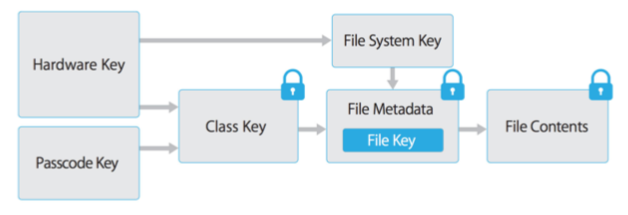
\includegraphics[width=\textwidth]{image17.png}
\caption {Secure Enclave Processor Scheme}
\label {fig01}
\end{figure}

 		A arquitetura é baseada numa hierarquia de chaves.
 		O User ID e uma passcode key que é derivada da aplicação do algoritmo PBKDF2 sobre a password de desbloqueio do dispositivo. 
 		Classkey está associada ao estado do dispositivo (bloqueado ou desbloqueado).
 		Cada ficheiro guardado no sistema de ficheiros está encriptado com uma chave por ficheiro.\par


Ficheiros têm 4 tipos de classes de proteção:

\begin{itemize}
\item \textit{Proteção completa:}
		A chave de classe é apagada da memória após o dispositivo ser bloqueado.Tornando os dados inacessiveis quando o dispositivo está bloquado.\par
		\hfill\par

\item \textit{Proteção até ser aberta:}
		Igual à anterior mas a chave não é apagada quando o dispositivo é bloqueado permitindo acesso ainda bloqueado. Útil para emails.\par
		\hfill\par
\item \textit{Proteçã até primeira autenticação do utilizador:}
		O ficheiro pode ser acedido mal o utilizador desbloqueie o dispositivo após liga-lo.\par
		\hfill\par
\item \textit{Sem proteção:}
		A chave de classe é guardado na \textit{Effaceable Storage\footnote[0]{A \textit{Effaceable Storage} é uma flash memory para pequenos dados que nunca é apagada.}}\par
\end{itemize}


Para realizarmos o teste ao armazenamento local, de forma a verificarmos se conseguimos aceder ao conteúdo dos dados basta seguirmos estes passos.

\begin{enumerate}
\item Acionar a funcionalidade da aplicação que guarda dados sensíveis, por exemplo fazer login na aplicação.

\item navegar até à diretoria com os ficheiros sensíveis.
\begin{lstlisting}
/var/mobile/Containers/Data/Application/$APP_ID/
\end{lstlisting}
\item executar grep com os dados guardados por exemplo: \textit{grep -iRn <USERID>}.

\end{enumerate}

Se os dados forem legiveis o teste falhou.


\subsubsection{Determinar se dados sensíveis são enviados para terçeiros (MSTG-STORAGE-4)}
\hfill\par
\hfill\par
Regras:
\begin{itemize}
\item Não deve ser enviada mais informação do que a estritamente necessária.
\item Todos os dados enviados para terceiros deve ser anonimizado para impedir exposição de PII (	Personal Identifiable Information).
\end{itemize}
Para realizar este teste basta usar um proxy para podermos intercetar o tráfico entre a aplicação e os terçeiros. Posteriormente podemos analisar o tráfico e se estiver a ser enviada informação sensivel pessoal, o teste falha.



\subsubsection{Procurar dados sensíveis na cache do teclado (MSTG-STORAGE-5)}
\hfill\par
\hfill\par

   O protocolo UITextInputTraits é usado para a cache do teclado e possui 2 propriedades: 
\begin{itemize}

   		\item \textit{var autocorrectionType UITextAutocorrectionType:} 

   			Determina se a correção automática está ativada durante a escrita, o valor por defeito desta propriedade é UITextAutocorrectionTypeDefault, que permite autocorreção. \par
   			\hfill\par

   		\item \textit{var secureTextEntry:}

   			Variável responsável por definir se se mantêm as palavras escritas em cache e se se escondem as palavras escritas nos campos UITextField. Por defito é NO.
\end{itemize}


   	O objetivo deste teste é procurar no código fonte da aplicação uma implementação semelhante à da figura para os UITextFields visados. Se estes não tiverem a configuração mostrada falham o teste.

\begin{figure}[H]
\centering
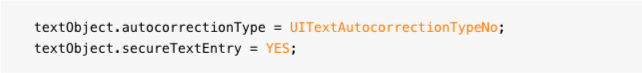
\includegraphics[width=\textwidth]{image26.png}
\caption {Secure Text Entry Example}
\label {fig02}
\end{figure}



Para corrigir este problema podemos programar uma solução para o UITextField alvo apicando o código: \textit{textObject.autocorrectionType = UITextAutocorrectionTypeNo} aos \textit{UITextFields}, \textit{UITextViews} e \textit{UISearchBars} que desejarmos. Para objetos que devem ser mascarados devemos definir o atributo \textit{textObject.secureTextEntry} como \textit{YES}.  Na imagem abaixo vemos um exemplo.
	 
\begin{figure}[H]
\centering
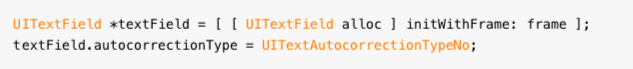
\includegraphics[width=\textwidth]{image27.png}
\caption {Set a secure Text Entry}
\label {fig02}
\end{figure}

Para testar se a cache do teclado possui dados sensiveis que não deveriam ser guardados, basta:
\begin{enumerate}
	\item Fazer reset à cache do teclado.
	\item Entrar na aplicação e inserir, por exemplo, os dados de autenticação.
	\item Sair da aplicação.
	\item Reentrar na aplicação e começar a reinserir os dados. 
	\item Se for permitido completar automáticamente o preenchimento dos dados, o teste falha.
\end{enumerate}



\subsubsection{Procurar exposição de dados sensíveis na interface do utilizador (MSTG-STORAGE-7)}
\hfill\par
\hfill\par


A inserção de informação sensível é necessária quando queremos por exemplo levantar dinheiro, fazer um pagamento entre outros. Ao utilizar aplicações que requerem esse tipo de dados sensíveis é imperativo que estes não sejam mostrados em texto limpo na interface após inseridos.\par
\hfill\par
Um campo que mascare o que nele é escrito pode ser verificado de duas formas.
A primeira pode ser verificada navegando pelo código da aplicação até à configuração da caixa que recebe os dadso sensíveis e verificando se a opção \textit{Secure Text Entry} está ativa, se estiver ativa o texto inserido é substituido por pontos.
A segunda é em interação com a aplicação a testar inserir os dados sensiveis e verificar se os dados aparecem em texto limpo ou são mascarados.



\subsection{iOS Cryptographic APIs}

\hfill\par

\subsubsection{Verificação da configuração dos algoritmos criptográficos standard (MSTG-CRYPTO-2 and MSTG- CRYPTO-3)}
\hfill\par
\hfill\par

O CriptoKit da Apple tem os seguintes algoritmos:
\begin{itemize}
\item \textit{Hashes:}

\begin{figure}[H]
\centering
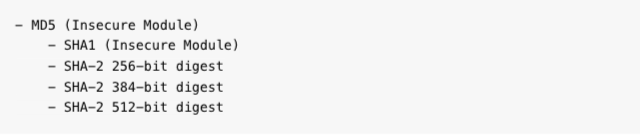
\includegraphics[width=\textwidth]{image38.png}
\caption {Available Hash Algorithms}
\label {fig02}
\end{figure}

\item \textit{Symmetric-Key:}

\begin{figure}[H]
\centering
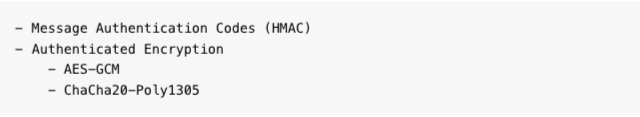
\includegraphics[width=\textwidth]{image39.png}
\caption {Available Symmetric-key Algorithms}
\label {fig02}
\end{figure}
\item \textit{Public-Key:}

\begin{figure}[H]
\centering
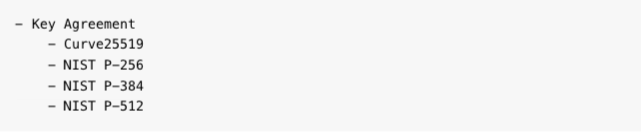
\includegraphics[width=\textwidth]{image40.png}
\caption {Available Public-key Algorithms}
\label {fig02}
\end{figure}
\end{itemize}

Se a aplicação usar implementações fornecidas no kit, a melhor forma de verificar o estado do algoritmo é analizando as chamadas ás funções do CommonCryptor. 

\begin{figure}[H]
\centering
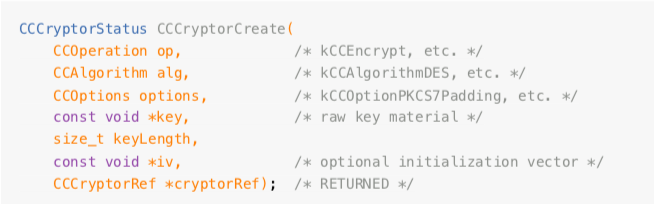
\includegraphics[width=\textwidth]{image41.png}
\caption {CommonCryptor Status}
\label {fig02}
\end{figure}

Podemos depois comparar os enums para determinar o algoritmo, o padding e a chave usados.
Após determinarmos os 3 podemos verificar se estes são seguros ou se já estão ultrapassados.



\subsubsection{Testar Gestão de Chaves (MSTG-CRYPTO-1 and MSTG-CRYPTO-5)}
\hfill\par
\hfill\par
Quando guardamos uma chave é recomendado o uso do keyChain desde que não se use o atributo kSecAttrAccessibleAlways.

O mecanismo de keyChain permite 2 formas de guardar chaves:
\begin{enumerate}
	\item Usar uma chave de segurança guardada no secure-enclave para encriptar a chave.

	\item Guardar a chave no secure-enclave\footnote[4]{ O Secure-enclave é um gestor de chaves baseado em hardware e isolado do processador para maior segurança\cite{book}.}.
\end{enumerate}



O teste tem de ser monitorizado verificando o acesso aos ficheiros do sistema durante operações criptográficas da aplicação.

O teste falha se:

	- Chaves usadas para proteger dados sensíveis são sincronizadas entre dispositivos.

	- Chaves não são guardadas com proteção.

	- Chaves não são derivadas de funcionalidades estáveis do dispositivo.

	- Chaves não são escondidas ao usar linguagens de baixo nivel.

	- Chaves são importadas de locais inseguros.




\subsubsection{Testar Geração Aleatória de Números (MSTG- CRYPTO-6)}
\hfill\par
\hfill\par

A Apple fornece uma API para gerar números aleatório criptográficamente seguros.

Em Swift a chamada à API é feita com o seguinte código:

\begin{lstlisting}[basicstyle=\small,]
    func SecRandomCopyBytes(_ rnd: SecRandomRef?,
                      _ count: Int,
                      _ bytes: UnsafeMutablePointer<UInt8>) -> Int32
\end{lstlisting}

 
A versão em Objective-C é:
\begin{lstlisting}[basicstyle=\small,]
 int SecRandomCopyBytes(SecRandomRef rnd, size_t count, uint8_t *bytes);
\end{lstlisting}
Um exemplo de utilização é:
\begin{lstlisting}[basicstyle=\small,]
  int result = SecRandomCopyBytes(kSecRandomDefault, 16, randomBytes);
\end{lstlisting}

Para testar se a implementação usada é segura basta verificar que a geração de números aleatórios, se não for igual ás acima descritas, sejam wraplicaçãoers implementados sobre a API acima. 

\textit{Nota: Podemos usar o plugin \textbf{Burp's sequencer} para avaliar a qualidade da geração dos números.}


\subsection{Local Authentication on iOS}
\hfill\par
Durante a autenticação local, uma aplicação autentica um utilizador verificando con credenciais guardadas localmente no dispositivo (PIN, password, carateristicas biometricas).

Atacantes podem facilmente passar a autenticação local caso nada seja retornado do processo de autenticação.


\subsubsection{Testar Autenticação Local (MSTG-AUTH-8 and MSTG-STORAGE-11)}
\hfill\par
\hfill\par
É importante lembrar que a framework de autenticação local é um processo baseado em eventos e portanto não deve ser o único método de autenticação.\par
\hfill\par


Apesar de ser uma autenticação eficiente ao nivel do utilizador, esta é facilmente ultrapassável usando instrumentos de patching. Assim é melhor usar o método de serviço da keyChain, ou seja, verificar que processos sensíveis são protegidos com métodos de serviço da keyChain. ex: transações financeiras.\par

Verificar as flags dos controlos de acesso da keyChain para assegurar que os dados só são acedidos pelo utilizador. Podem-se utilizar as seguintes flags: 

\begin{itemize}

\item \textit{kSecAccessControlBiometryCurrentSet:}\par
	\hfill\par
	Esta flag obriga o utilizador a autenticar-se biometricamente antes de aceder à keyChain. Se for adicionado um novo dado biométrico, a entrada na keyChain vai ser invalidada e só poderá ser acedida pelos utilizadores autenticados quando os dados foram adicionados.\par
	\hfill\par

\item \textit{kSecAccessControlBiometryAny:}\par
	\hfill\par
	Esta flag obriga o utilizador a autenticar-se biometricamente antes de aceder à keyChain. Caso novos dados biométricos sejam adicionados a autenticação na keyChain mantem-se. Útil para utilizadores que mudam a própria impressão digital mas bom para atacantes também visto que se conseguirem registar a impresão digital conseguem aceder aos restantes dados biométricos.\par
	\hfill\par

\item \textit{kSecAccessControlUserPresence:}\par
	\hfill\par
	Permite que o utilizador se autentique por password se autenticação biométrica não funcionar. É mais fraco visto ser mai facil roubar uma password por shouldersurfing do que passar pelso dados biométricos.
\end{itemize}

Para garantir que os dados biométricos podem ser usados temos de verificar se a classe kSecAttrAcessibleWhenPasscodeSetThisDeviceOnly ou a kSecAttrAcessibleWhenPasscodeSet estão implementadas\footnote[5]{A variante ThisDeviceOnly garante que não há sincronização dos dados biométricos entre dispositivos iOS.}.\par
\hfill\par

Para um dispositivo \textit{jailbroken} existem ferramentas que permitem efetuar uma quebra na segurança da autenticação local. Neste exemplo usaremos o Swizzler2, uma ferramenta que através do uso do software Frida permite que a função de autenticação retorne True mesmo que tenha falhado.\par
\hfill\par
Os passos para efetuar o teste são:
\begin{enumerate}
\item Ir aos settings e escolher Swizzler
\item Permitir injeção do Swizzler nas aplicações
\item Permitir registar tudo no Syslog
\item Permitir registar tudo num ficheiro
\item Entrar nos submenus da framework iOS
\item Permitir autenticação local
\item Entrar no submenu e escolher as aplicações alvo
\item Permitir que a aplicação escolhida corra
\item Reiniciar a aplicação
\item Quando for pedida a impressão digital carregar em cancelar
\end{enumerate}

Se a aplicação continuar sem requerer a impressão digital esta não passou no teste.



\subsection{iOS Network APIs}
\hfill\par
Quase todas as aplicações no iOS atuam como cliente de um ou mais serviços remotos.  Como não podemos confiar nas redes pública. Temos portanto de garantir que as aplicações tomam medidas para mitigar os riscos. 


\subsubsection{Segurança da Camada de Trasporte da Aplicação (MSTG-NETWORK-2)}
\hfill\par
\hfill\par
 A App Transport Security (ATS) é um conjunto de verificações de segurança que o sistema operativo realiza quando efetua conecções com NSURLConnection\footnote[6]{ Conecções NSURLConnection permitem carregar conteúdos de um URLao fornecer um pedido para um objeto URL\cite{ref_intro4}.}, NSURLSession\footnote[7]{A classe NSURLSession fornece uma API para download e para upload de dados entre pontos opostos de uma conexão indicados por URLs\cite{ref_intro5}.} e CFURL\footnote[8]{ O tipo CFURL fornece facilidade para criar, percorrer e desreferenciar strings URL\cite{ref_intro6}.} a servidores públicos. Estas verificações são efetuadas por defeito do iOS SDK 9 em diante.\par
Quando a ligação é feita a um IP, um dominio de nomes não qualificado ou TLD de .local o ATS não é aplicado.\par
\hfill\par
Agora vamos ver uma análise das configurações da ATS.\par

Se o código fonte estiver disponivel devemos abrir a Info.plist na diretoria da aplicação (\textit{Bundle Directory}) que o desenvolvedor configurou. Na imagem abaixo vemos um exemplo de uma exceção configurada para desativar as restrições globais da ATS.

\begin{figure}[H]
\centering
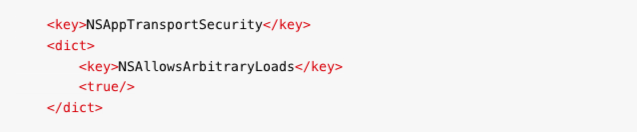
\includegraphics[width=\textwidth]{image42.png}
\caption {ATS example configuration}
\label {fig02}
\end{figure}

A desativação das restrições da ATS depende da aplicação, por exemplo a aplicação do chrome para iOS tem estas configurações, o que é aceitavel visto que por outro lado a aplicação não se conseguiria ligar a um site HTTP que não tivesse todos os requisitos da ATS.

As recomendações para o uso da ATS são:
\begin{itemize}
\item A ATS deve ser configurada de acordo com as melhores práticas aconcelhadas pela Apple e só deve ser desativada excecionalmente.\par
\hfill\par
\item Se a aplicação se conectar a um número definido de dominios que o dono da aplicação controla, esses dominios devem suportar a ATS.\par
\hfill\par
\item Se houver conecções a terçeiros (que não pertençam ao dono da aplicação) devem ser avaliados quais os requisitos da ATS que não são suportados e podem ser desativados.\par
\hfill\par
\item Se a apicação abrir sites web de terçeiros, do iOS 10 para a frente pode-se usar o \textit{NSAllowsArbitraryLoadsInWebContent} para desabilitar as restrições da ATS para o conteúdo das páginas web.
\end{itemize}

\subsubsection{Teste e Validação de Certificados (MSTG-NETWORK-3 and MSTG-NETWORK-4)}
\hfill\par
\hfill\par

As autoridades de cetificação são uma parte fulcral da comunicação cliente-servidor. No iOS existem uma quantidade enorme de certificados confiáveis. CAs podem ser adicionadas manualmente pelo utilizador ou por malware, para precaver esta situação basta  remover a confiança nas CAs adicionadas.\par
Falhas podem ocorrer se a aplicação esperar outra chave ou certificado do servidor, ou pode estar a ocorrer um ataque.
Nestes casos basta seguir os passos referidos no capitulo \textit{Android Network APIs}\cite{book}.\par
\hfill\par
Em baixo apresentamos 3 formas de manter os certificados confiaveis por parte da aplicação.
\begin{enumerate}
\item Incluir os certificados do servidor na diretoria da aplicação e verifica-lo a cada conecção. Isto requer um mecanismo de atualização do certificado para o caso do certificado mudar.\par
\hfill\par
\item Limitar os emissores de certificados, ex: uma CA envia à aplicação o certificado de um servidor. O certificado será seguro e limita ataques possíveis.\par
\hfill\par
\item A aplicação deve possuir a chave pública da CA confiavel pertencente ao dono da aplicação. Isto não requer atualizar a aplicação sempre que o servidor mudar de certificado. Usar uma CA própria faz com que o seu certificado seja auto assinado.
\end{enumerate}

Para validarmos os certificados presentes na aplicação vamos usar o Burp para intercetar o tráfico que circula entre a aplicação a testar e o seridor a que esta se está a ligar. Posteriormente realizamos os seguintes passos pela ordem em que aparecem.

\begin{enumerate}
\item Temos de verificar se ferramentas como o SSL Kill Switch estão desativadas.\par
\hfill\par
\item Garantir que não há certificados a serem adicionados à diretoria da aplicação.\par
\hfill\par
\item Iniciar a aplicação, se conseguirmos ver o tráfico não é realizada nenhuma validação do certificado e a aplicação falhou o teste.\par
\hfill\par
\item Se houver uma falha no SSL handshake (está a ser verificada a validade do certificado), instalamos o certificado do  Burp.\par
\hfill\par
\item Se o handshake for bem sucedido e conseguimos ver o tráfico, o certificado foi validado com o certificado na diretoria da aplicação mas não pela cadeia de confiança da mesma. A aplicação falha neste ponto se tal ocorrer.
\end{enumerate}


Se não conseguirmos ver o tráfico apesar do SSL handshake funcionar então todas as medidas de segurança para o establecimento da conecção foram tomadas e a aplicação passou no teste.


\subsection{iOS Platform APIs}
\hfill\par


\subsubsection{Testar Permissões das Aplicações (MSTG-PLATFORM-1)}
\hfill\par
\hfill\par

Ao contráro do android  cada aplicação no iOS corre sobre o seu ID de utilizador, todas as aplicações de terçeiros correm sobre o non-privileged mobile user.

Algumas permissões no entanto podem ser configuradas pelo desenvolvedor da aplicação e terão efeito mal a aplicação seja instalada. Este é o problema que trataremos nesta secção, aplicaçãos que pedem permissões por razões não obvias, pr exemplo um scanner de QRcodes deve ter acesso à câmara mas dificilmente necessitará de acesso ás fotografias.\par
\hfill\par

Desde o iOS 10 existem areas que precisam de inspeção ás permissões:
\begin{itemize}
\item \textit{Mensagens de permissões no ficheiro Info.plist}\par
\hfill\par
	Estas mensagens são as que aparecem por defeito quando a aplicação pretende ter acesso a um recurso.

\begin{figure}[H]
\centering
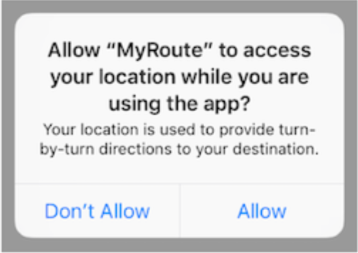
\includegraphics[width=0.5\textwidth]{image45.png}
\caption {Example of permission request message}
\label {fig02}
\end{figure}
	O objetivo de verificar o ficheiro é poder ler a justificação do uso da permissão por parte da aplicação como se pode ver na imagem abaixo.
\begin{figure}[H]
\centering
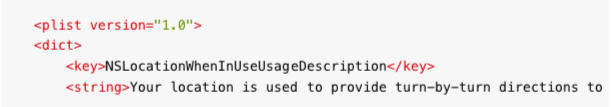
\includegraphics[width=\textwidth]{image46.png}
\caption {Example of permission request with justification}
\label {fig02}
\end{figure} 

\item \textit{Ficheiro de permissões do código da aplicação}\par
	\hfill\par

	Visualizar este ficheiro serve unicamente para verificar que a aplicação não pede permissões demasiado elevadas para o que tem de fazer permitindo assim fugas de dados.
	Na imagem abaixo podemos ver o exemplo da permissão pedida pela aplicação Telegram (aplicaçãolication-groups). Esta aplicação passa no teste por não pedir permissões adicionais, visto que não tem necessidade destas.

\begin{figure}[H]
\centering
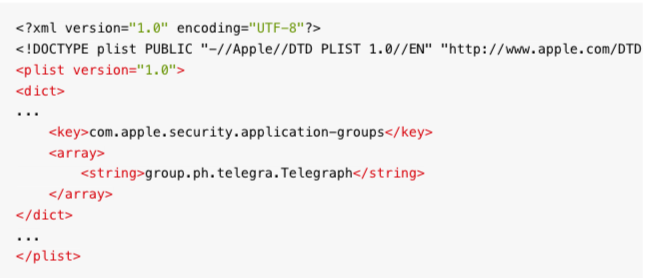
\includegraphics[width=\textwidth]{image47.png}
\caption {Example of Telegram's permission request}
\label {fig02}
\end{figure}

\item \textit{Permissões incluidas nos ficheiros binarios compilados}\par
\hfill\par
	Mais uma vez vamos procurar por permissões.
	Podemos usar a aplicação radare2 (com -qc para correr o comando e sair sem deixar registos) para procurar em todas as strings dos ficheiros binario por \textit{PropertyList} como podemos ver no exemplo abaixo.

\begin{figure}[H]
\centering
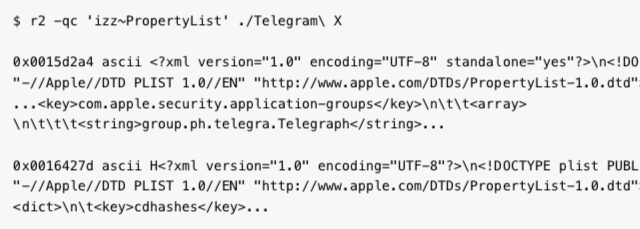
\includegraphics[width=\textwidth]{image48.png}
\caption {Result of searching for PropertyList with radare2}
\label {fig02}
\end{figure}

\item \textit{Inspeção do código fonte}\par
\hfill\par
	Esta inspeção tem de ser feita para verificar se as permissões são usadas corretamente. Assim as recomendações são:\par
	\hfill\par
	\begin{itemize}
		\item Verificar se as strings que explicam a razão pela qual a aplicação precisa da permissão e a forma como a aplicação usa essa permissão são compatíveis.\par
		\hfill\par
		\item Verificar que as permissões concedidas não são usadas para divulgamento de dados pessoais.
	\end{itemize}
\end{itemize}



\subsubsection{Testar Exposição de Dados Sensiveis através de Funcionalidades IPC (MSTG-PLATFORM-4)}
\hfill\par
\hfill\par

Durante a implementação de uma aplicação os desenvolvedores podem usar técnicas tradicionais para o IPC (como ficheiros ou sockets partilhadas), as funcionalidades do IPC para aplicações devem ser usadas visto serem muto mais seguras para não haver comprometimento de dados.\par
\hfill\par

Testar um link universal requer os seguintes passos:
\begin{enumerate}

\item \textit{Verificar as permissões do dominio associado}\par
\hfill\par
	Links universais requerem que o desenvolvedor adicione as permissões dos dominios associados numa lista de dominios que a aplicação suporte.
	Podemos usar o Xcode para verificar isto. Basta ir a \textit{Capabilities} e procurar por \textit{Associated Domains}. Em baixo mostra-se um exemplo com recurso à inspeção da aplicação Telegram.

\begin{figure}[H]
\centering
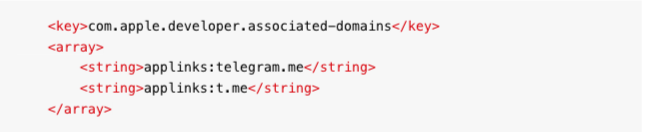
\includegraphics[width=\textwidth]{image49.png}
\caption {Example of domain permission request for universal link usage}
\label {fig02}
\end{figure}

\item \textit{Obter o ficheiro de associação no site da Apple}\par
\hfill\par

	Este ficheiro tem de ser acessivel por HTTPS sem redirecionamentos em \textit{https://<domain>/.well-known/aplicaçãole-aplicação-site-assosiation}.

	Se tudo correr bem o site verificará por nós que o link é seguro e apresentará um relatório semelhante ao mostrado.

\begin{figure}[H]
\centering
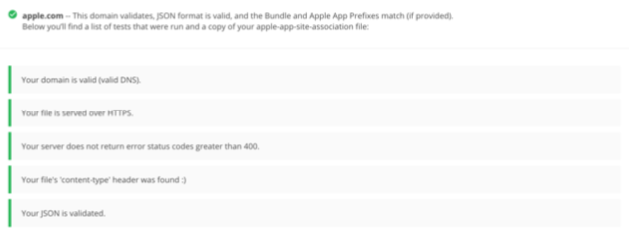
\includegraphics[width=\textwidth]{image50.png}
\caption {Safe link verifyed}
\label {fig02}
\end{figure}
	

\item \textit{Verificar o método de recepção do link}\par
\hfill\par

	Para receber o link e trata-lo de forma apropriada a aplicação tem de implementar a \textit{aplicaçãolication:continueUserActivity:restorationHandler:}. Devemos portanto procurar este método para garantir que a aplicação passa o teste.\par

	Adicionalmente, quando a aplicação usar o método \textit{openURL:options:completionHandler:} para abrir o link universal devemos verificar se o esquema da página URL é  HTTP or HTTPS. Caso nã seja, se não for lançada uma excepção a aplicação falha o teste.\par
\hfill\par

\item \textit{Verificar o método de processamento de dados}\par
\hfill\par

	Devemos verificar como são validados os dados recebidos visto que uma má verificação fornece um vetor de ataque a terçeiros. Assim todos os parâmetros fornecidos no URL não devem ser aceites sem antes serem validados.  
	A API NSURLComponents pode ser usada para verificar e manipular os componentes do URL.
	Por fim deve ser verificado que as ações requeridas pelo URL não expõem dados sensíveis.\par
\hfill\par


\item \textit{Verificar se a aplicação está a usar os links universais de outra aplicação}\par
\hfill\par

	Uma aplicação pode utilizar links de outra aplicação para transferir informação ou desencadiar alguma ação especifica, neste caso devemos garantir que não há vazamento de informação.
	Podemos para isso procurar o método \textit{openURL:options:completionHandler:} e verificar os dados manipulados.
	Em baixo temos um exemplo do que foi descrito em cima. Para este exemplo usamos o rabin2 para procurar nos ficheiros binários da aplicação.\par

\begin{figure}[H]
\centering
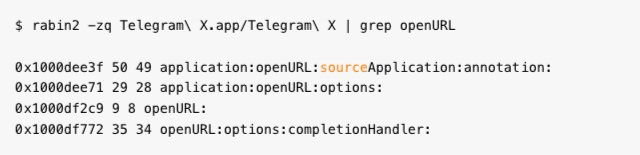
\includegraphics[width=\textwidth]{image51.png}
\caption {Result of searching for \textit{openURL:options:completionHandler:} with rabin2}
\label {fig02}
\end{figure}

	Note-se que a aplicação adapta o link para HTTPS antes de o usar e como só usa o URL caso este seja um link universal válido e só o abre caso haja uma aplicação capaz de o abrir.\par

	Como esperado o método \textit{openURL:options:completionHandler:} está implementado. Agora basta-nos garantir que dados sensíveis não são trocados entre as aplicações.\par

	Para imprimir os dados tansmitidos vamos usar o comando:
	\begin{lstlisting}[basicstyle=\small,]
 $ xcrun swift-demangle S10TelegramUI15openExternalUrl7account7
 context3url05for18applicationContext20navigationController12di
 smissInputy0A4Core7AccountC_AA1412PresentationK0CAA0a11Applica
 tionM0C7Display010NavigationO0CSgyyctF
	 \end{lstlisting}
	 Este comando apenas imprime o método \textit{TelegramUI.openExternalUrl} sem os parâmetros que lhe são passados, para que imprima mais do que isso temos de fazer alguns ajustes.\par
\hfill\par

	Primeiro vamos imprimir os parâmetros passados, alterando o ficheiro stub com se vê na imagem e o respetivo resultado de voltar a correr o comando anterior.

\begin{figure}[H]
\centering
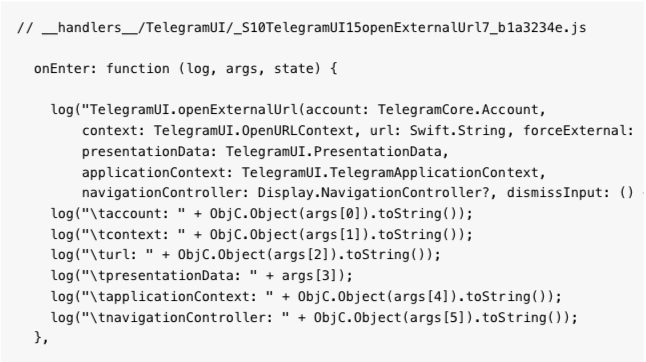
\includegraphics[width=\textwidth]{image52.png}
\caption {Code to print the parameters passed to \textit{TelegramUI.openExternalUrl}}
\label {fig02}
\end{figure}

\begin{figure}[H]
\centering
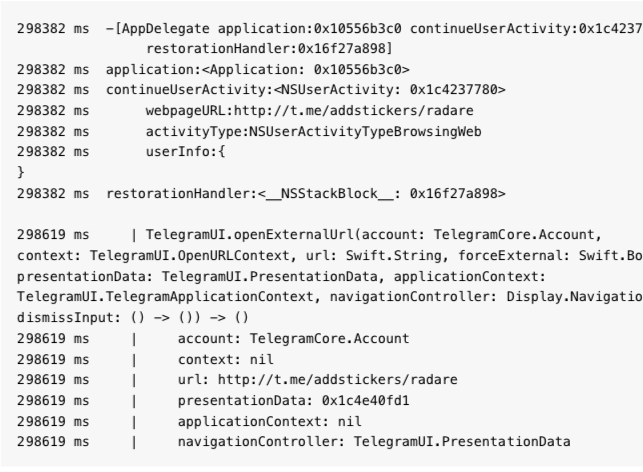
\includegraphics[width=\textwidth]{image53.png}
\caption {Parameters passed to \textit{TelegramUI.openExternalUrl}}
\label {fig02}
\end{figure}

		Aqui podemos observar que de facto o Telegram chama o método "aplicaçãolication:continueUserActivity:restorationHandler:" como esperado e que apenas trata o URL sem o abrir, chamando o \textit{TelegramUI.openExternalUrl} para isso.\par
\hfill\par

	Agora que confirmamos que o Telegram está a aplicar os métodos corretamente falta ver se temos dados sensíveis a serem trocados entre aplicações. Para isso, basta adicionar ao ficheiro stub o seguinte código: "log("userInfo:" + ObjC.Object(args[3]).userInfo().toString())". Este código  permite aceder à propriedade userInfo a partir do objeto continueUserInfo e como consequência imprime todos os dados trocados nos quais podemos verificar se existem ficheiros sensíveis.
	Na imagem seguinte vemos que não há dados sensíveis a serem passados.
	
\begin{figure}[H]
\centering
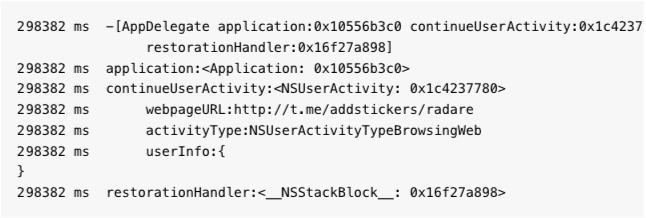
\includegraphics[width=\textwidth]{image54.png}
\caption {Print proving the safe implementation of Telegram}
\label {fig02}
\end{figure}
\end{enumerate}




\subsection{App Extensions}
\hfill\par
Para podermos analisar quais os testes a fazer temos primeiro de compreender o que são as extensões e como interagem com as aplicações.

Dependendo da tarefa, a extensão da aplicação vai ter um tipo especifico (apenas 1), o chamado ponto de extensão. Alguns exemplos são:
\begin{itemize}
\item \textit{Teclado personalizado:} substitui o teclado por um teclado personalizado para usar em todas as aplicaçãos.\par
\hfill\par

\item \textit{Partilha:} postagem para um site ou partilha de conteudos com terceiros.\par
\hfill\par

\item \textit{Hoje:} conhecidos como \textit{widgets}, oferecem conteudo ou realizam tarefas rápidas no centro de notificações.
\end{itemize}
A forma de interação com outras aplicações também pode variar:
\begin{itemize}
\item \textit{App extension:} É a extensão confinada dentro de uma aplicação. As aplicações de terceiros usam esta extensão.\par
\hfill\par

\item \textit{Host aplicação:} Trata-se da aplicação de terceiros que usa a extensão de outra aplicação.\par
\hfill\par

\item \textit{Containing aplicação:} Trata-se da aplicação que contem a extensão da aplicação instalada nela. \par
\hfill\par
\end{itemize}
Para melhor se percecionar a interação entre aplicações apresenta-se a imagem seguinte.

\begin{figure}[H]
\centering
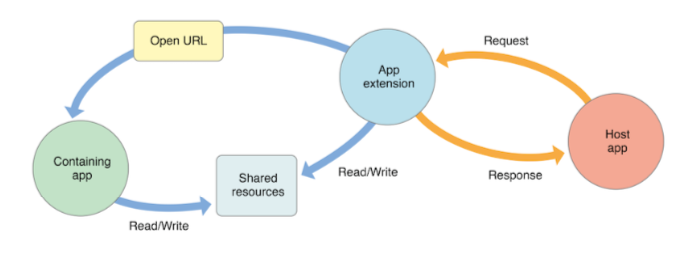
\includegraphics[width=\textwidth]{image55.png}
\caption {Aplication's shared URL implementation}
\label {fig02}
\end{figure}



\subsubsection{Determinar Exposição de Métodos Nativos através de WebViews (MSTG-PLATFORM-7)}
\hfill\par
\hfill\par

Desde o iOS a Apple introduziu APIs que permitem a comunicação entre o JavaScript na página web e o Swift ou Objective-C.
Se as APIs forem usadas de forma descuidada funcionalidades podem ser expostas através de ataques de Cross-Site Scripting.\par

Vamos então testar a UIWebView do JavaScript. Para a testarmos temos de compreender que há 2 formas fundamentais para a comunicação do JavaScript:
\begin{itemize}
	\item\textit{JSContext:} Quando é atribuido um identificador a um bloco Swift ou Objective-C num contexto JSContext, o bloco é envolto em uma função JavaScript.  \par
\hfill\par

	\item\textit{JSExport protocol:} métodos de instancia e de classes declarados no JSExport são mapeados para objetos JavaScript globais. Modificações aos objetos JavaScript são refletidas no ambiente nativo. \par
\hfill\par
\end{itemize}

Devemos portanto verificar o código que resulta do mapeamento para o JSContext para ver que funcionalidades são expostas para garantir que dados sensíveis não podem ser acedidos e expostos na WebView. \par
\hfill\par
Em Objective-C o JSContext associado a uma 	UIwebView pode-se obter com o comando:
\begin{lstlisting}[basicstyle=\small,]
[webView valueForKeyPath:@"documentView.webView.mainFrame.javaScriptContext"]
\end{lstlisting}


Para testarmos as funções devemos produzir código JavaScript para injetar num ficheiro que a aplicação utilize. Podem ser aplicadas várias técnicas para realizar isto. Vamos apresentar duas:
\begin{enumerate}

\item Se algum do conteúdo for carregado de forma insegura da internet por HTTP, podemos tentar implementar um ataque man-in-the-middle onde fornecemos o nosso código. \par
\hfill\par

\item Podemos realizar uma injeção do código ao usar frameworks como a Frida e as funções de avaliação do javaScript correspondentes a cada WebView:
	\begin{enumerate}
		\item Usar "stringByEvaluatingJavaScriptFromString:" para a UIWebView \par
\hfill\par
		\item Usar "evaluateJavaScript:completionHandler:" para a WKWebView
	\end{enumerate}
\end{enumerate}
Para efeitos de demonstração foi usada uma aplicação chamada "where's My Browser?", que fornece um serviço de calculadora web e que possui um método que, quando chamado, devolve um segredo (informação sensivel).\par
\hfill\par
Para expor o segredo da aplicação "where's My Browser?" podemos usar uma das técnicas mencionadas para injetar o seguinte código:

\begin{lstlisting}[basicstyle=\small,]
function javascriptBridgeCallBack(name, value) {
	  document.getElementById("result").innerHTML=value;
};

window.webkit.messageHandlers.javaScriptBridge.postMessage(["getSecret"]);
\end{lstlisting}
O resultado pode ser visto na imagem seguinte.

\begin{figure}[H]
\centering
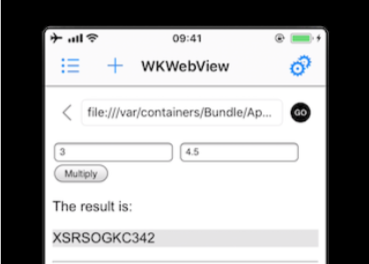
\includegraphics[width=0.5\textwidth]{image56.png}
\caption {Leaked Secret through javaScript code injection}
\label {fig02}
\end{figure}


\subsubsection{Testar Updates Forçados (MSTG-ARCH-9)}
\hfill\par
\hfill\par

Este teste tem por base a realização de updates. Como a Apple ainda não fornece uma API para automatizar o processo de atualização de aplicações os desenvolvedores terão de o programar.\par
\hfill\par

A primeira coisa a ser verificada é a presença de um mecanismo de atualização. Sem este os utilizadores não serão forçados a atualizar a aplicação.\par
Caso haja o dito mecanismo temos de verificar se este força a atualizar para "always latest". Temos também de verificar que de cada vez que se inicia a aplicação, esta passa pelo mecanismo de update para garantir que o mecanismo não pode ser ultrapassado.\par
\hfill\par

Para testar o mecanismo devemos tentar instalar uma versão da aplicação que tenha uma vulnerabilidade. De seguida devemos iniciar a aplicação e verificar se esta corre ou se nos obriga a atualizar. Se uma janela de atualização for mostrada temos de verificar se fechando-a conseguimos continuar a correr a aplicação e, caso esta continue a correr, se o backend está preparado para não nos permitir aproveitar a vulnerabilidade bloqueando-nos o acesso enquanto a aplicação não for atualizada.\par

Se todas as tentativas para explorar a vulnerabilidade falharem a aplicação foi bem sucedida.




%
% ---- Bibliography ----
%
% BibTeX users should specify bibliography style 'splncs04'.
% References will then be sorted and formatted in the correct style.
%
% \bibliographystyle{splncs04}
% \bibliography{mybibliography}
%

\begin{thebibliography}{8}

%regra de adição exemplo

\bibitem{ref_intro1} https://www.theiphonewiki.com/wiki/DFU\_Mode
\bibitem{ref_intro2} https://www.lifewire.com/what-is-jailbreaking-2377420
\bibitem{ref_intro3} https://mobile-security.gitbook.io/mobile-security-testing-guide/ios-testing-guide/0x06j-testing-resiliency-against-reverse-engineering
\bibitem{ref_intro4} https://developer.apple.com/documentation/foundation/nsurlconnection
\bibitem{ref_intro5} https://developer.apple.com/documentation/foundation/nsurlsession
\bibitem{ref_intro6} https://developer.apple.com/documentation/corefoundation/cfurl-rd7
\bibitem{book} Bernhard Mueller, Sven Schleier, Jeroen Willemsen, Carlos Holguera, The OWASP mobile team. MSTG - Mobile Security Testing Guide. The OWASP Foundation. 2 August 2019
\bibitem{ref_intro7} https://owasp.org/www-community/Application\_Threat\_Modeling
\bibitem{ref_intro8} https://owasp.org/www-project-top-ten/
\bibitem{ref_intro9} https://cheatsheetseries.owasp.org/cheatsheets/Authentication\_Cheat\_Sheet.html
\bibitem{ref_intro10} https://owasp.org/www-community/controls/Blocking\_Brute\_Force\_Attacks
\bibitem{ref_intro11} https://wiki.owasp.org/index.php/Testing\_for\_authentication
\bibitem{ref_intro12} https://wiki.owasp.org/index.php/Testing\_for\_Session\_Management

\end{thebibliography}
\end{document}
